% !TEX root = thesis.tex
\chapter{Feature Selection}
\label{app:feature_selection}
In Section~\ref{sec:conclusions_contributions} we mentioned the we can reduce the used feature sets using a technique call \emph{feature selection}. With feature selection it is possible to minimize the loss or possibly increase the predictive performance, and reduce cost (with respect to time and space). This appendix was originally planned for the optimization section (Section~\ref{subsec:experiment_optimization_generalization}) though we decided to move this section in an appendix as the results were not significant.

In machine learning one typically gathers as many features as possible to supply sufficient data such that the learning algorithms can make accurate predictions. The general problem is to predict the correct category based on a vector, in some cases there are redundant, irrelevant or detrimental features to the predictive efforts. With the right set of features, the prediction performance can improve, or remain the same with less information required. With a reduced feature load, the actual performance (i.e., with respect to computational resources required) will improve. Feature selection makes it is possible to utilize a subset of the initially defined feature set that improve/maintain the predictive performance while requiring less data~\cite{GE03,BL97}.

There are several approaches to feature selection, in particular \emph{filter} and \emph{wrapper}. Filters assess the quality/merits of features solely from the data alone as a preprocessing step~\cite{JKP94,BL97}. Various algorithms and measures can be used as a filter (i.e., information gain~\cite{GE03}, correlation~\cite{Hal99}, \emph{FOCUS}~\cite{AD91}, \emph{Relief}~\cite{KR92}, etc\ldots). An alternative to filters are wrappers, which evaluates the actual performance of features using the classifier. Wrappers treat the classifier as a black-box and assess the performance using various subsets of features by using the actual predictor~\cite{JKP94,BL97}. Wrappers provide a more accurate and effective means in finding appropriate features, though inefficient as the classification process must occur many times using cross-validation with different features~\cite{KJ97}.

We have over 3000 vectors (with undersampling in effect) with 15 features for the method-level data set (see Table~\ref{tab:metrics}). A wrapper approach could be very costly in our situation, though might prove more effective as found by Kohavi and John~\cite{KJ97}. For our research we decided against a wrapper approach due to the high computational cost involved. As an alternative to a wrapper approach we use Hall's \emph{\gls{cfs}} filter which is based on the follow definition: \emph{``A good feature subset is one that contains features highly correlated with (predictive of) the class, yet uncorrelated with (not predictive of) each other''}~\cite{Hal99}. We used Hall's \gls{cfs} implementation found in the machine learning toolkit \emph{WEKA}~\cite{HFH+09}.

To further investigate Hall's filter we created a correlation matrix of our features along with the raw mutation score and used category for the source code unit. We discovered that none of our features are highly correlated with the predicted category. In the class-level correlation there were only six features (i.e., \emph{APAR}, \emph{ATNBD}, \emph{ATVG}, \emph{NOF}, \emph{NSC} and \emph{SPAR}) that had a correlation between 0.3 and 0.5 (i.e., moderate correlation) with the rest being weak or no correlation. In the method-level correlations \emph{ATMLOC} was the only feature with a moderate correlations while the rest were weak or no correlation. There were a number of features that are highly correlated with each other (e.g., size and complexity). These findings suggest either:

\begin{itemize}
  \item The selected features are insufficient in describing the predicted category.
  \item The difficulty of predicting the mutation score category is a highly complex process.
\end{itemize}

We believe that the observed correlations suggest the the prediction of the mutation score category is difficult. As mentioned in Section~\ref{sec:approach_process}, there are two source artifacts involved in determining the mutation score, and our features are both well established descriptive metrics of these source artifacts.

We used the available data of the \emph{all} data set (i.e., all the test subjects together) for both class- and method-level. Ten different undersampled data set of vectors that contain all our features were apply the \gls{cfs} filter to produce an ascending order of features with respect to their correlation ranking (i.e., how effective the feature is with respect to others). To account for the undersampling we apply the \gls{cfs} filter on each of the ten undersampled sets of data. We then use a simple rank summation to tally the results (i.e., ascending rank $n$ has a value of $n$, and so forth), which then allowed us to create overall ranking of the features across the ten different undersampled data sets. We then removed the least useful feature one at a time and observed the new $10$-fold cross-validation performance of the classifier using a subset of all the features.

\begin{figure}[ht!]
  \centering
  \begin{adjustbox}{max size={.95\textwidth}{.95\textheight}}
    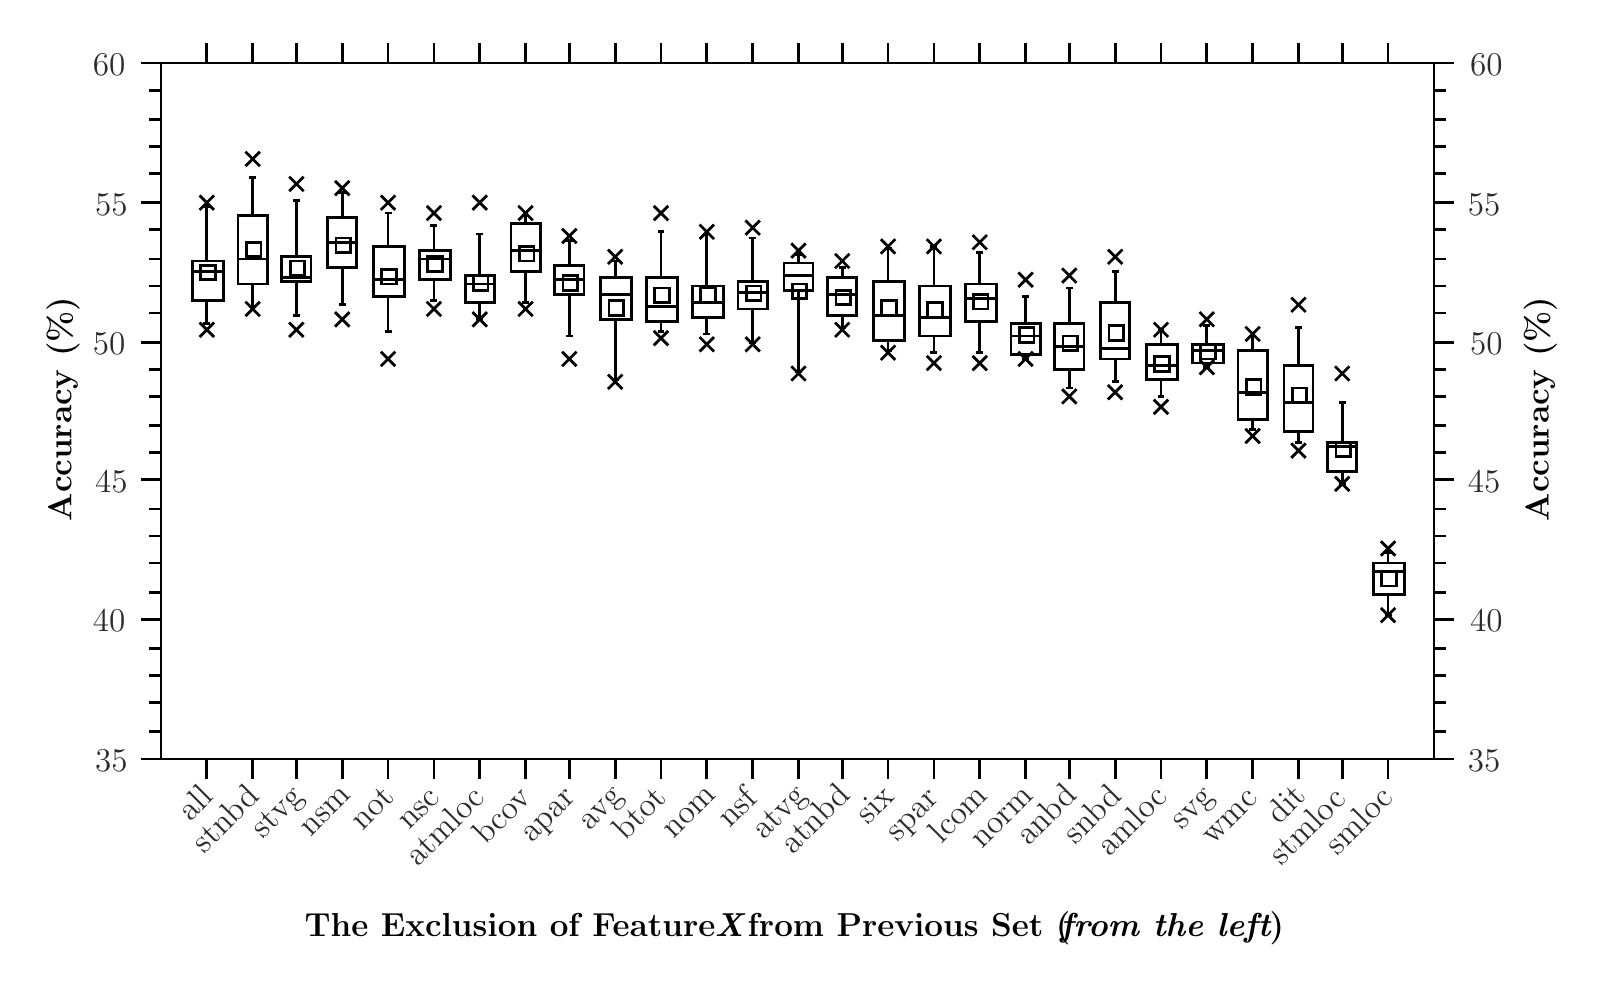
\begin{tikzpicture}{0pt}{0pt}{742pt}{452pt}
	\clip(0pt,452pt) -- (558.587pt,452pt) -- (558.587pt,111.729pt) -- (0pt,111.729pt) -- (0pt,452pt);
\begin{scope}
	\clip(48.18pt,439.202pt) -- (508.148pt,439.202pt) -- (508.148pt,187.763pt) -- (48.18pt,187.763pt) -- (48.18pt,439.202pt);
	\color[rgb]{0,0,0}
	\draw[line width=1pt, line join=miter, line cap=rect](59.4722pt,367.685pt) -- (70.7644pt,367.685pt) -- (70.7644pt,353.382pt) -- (59.4722pt,353.382pt) -- (59.4722pt,367.685pt);
	\color[rgb]{0,0,0}
	\draw[line width=1pt, line join=miter, line cap=rect](63.9891pt,345.101pt) -- (65.4947pt,345.101pt);
	\draw[line width=1pt, line join=miter, line cap=rect](63.9891pt,387.258pt) -- (65.4947pt,387.258pt);
	\draw[line width=1pt, line join=miter, line cap=rect](64.7419pt,387.258pt) -- (64.7419pt,367.685pt);
	\draw[line width=1pt, line join=miter, line cap=rect](64.7419pt,345.101pt) -- (64.7419pt,353.382pt);
	\draw[line width=1pt, line join=miter, line cap=rect](59.4722pt,363.921pt) -- (70.0116pt,363.921pt);
	\draw[line width=1pt, line join=miter, line cap=rect](62.4834pt,345.101pt) -- (67.0003pt,340.584pt);
	\draw[line width=1pt, line join=miter, line cap=rect](62.4834pt,340.584pt) -- (67.0003pt,345.101pt);
	\draw[line width=1pt, line join=miter, line cap=rect](62.4834pt,391.022pt) -- (67.0003pt,386.505pt);
	\draw[line width=1pt, line join=miter, line cap=rect](62.4834pt,386.505pt) -- (67.0003pt,391.022pt);
	\draw[line width=1pt, line join=miter, line cap=rect](62.4834pt,366.179pt) -- (67.7531pt,366.179pt) -- (67.7531pt,360.91pt) -- (62.4834pt,360.91pt) -- (62.4834pt,366.179pt);
	\draw[line width=1pt, line join=miter, line cap=rect](76.0341pt,384.247pt) -- (86.5734pt,384.247pt) -- (86.5734pt,359.404pt) -- (76.0341pt,359.404pt) -- (76.0341pt,384.247pt);
	\draw[line width=1pt, line join=miter, line cap=rect](80.5509pt,351.123pt) -- (82.0566pt,351.123pt);
	\draw[line width=1pt, line join=miter, line cap=rect](80.5509pt,397.798pt) -- (82.0566pt,397.798pt);
	\draw[line width=1pt, line join=miter, line cap=rect](81.3037pt,397.798pt) -- (81.3037pt,384.247pt);
	\draw[line width=1pt, line join=miter, line cap=rect](81.3037pt,351.123pt) -- (81.3037pt,359.404pt);
	\draw[line width=1pt, line join=miter, line cap=rect](76.0341pt,368.438pt) -- (86.5734pt,368.438pt);
	\draw[line width=1pt, line join=miter, line cap=rect](79.0453pt,352.629pt) -- (83.5622pt,348.112pt);
	\draw[line width=1pt, line join=miter, line cap=rect](79.0453pt,348.112pt) -- (83.5622pt,352.629pt);
	\draw[line width=1pt, line join=miter, line cap=rect](79.0453pt,406.831pt) -- (83.5622pt,402.314pt);
	\draw[line width=1pt, line join=miter, line cap=rect](79.0453pt,402.314pt) -- (83.5622pt,406.831pt);
	\draw[line width=1pt, line join=miter, line cap=rect](79.0453pt,374.46pt) -- (84.315pt,374.46pt) -- (84.315pt,369.191pt) -- (79.0453pt,369.191pt) -- (79.0453pt,374.46pt);
	\draw[line width=1pt, line join=miter, line cap=rect](91.8431pt,369.191pt) -- (102.382pt,369.191pt) -- (102.382pt,360.157pt) -- (91.8431pt,360.157pt) -- (91.8431pt,369.191pt);
	\draw[line width=1pt, line join=miter, line cap=rect](96.36pt,348.112pt) -- (97.8656pt,348.112pt);
	\draw[line width=1pt, line join=miter, line cap=rect](96.36pt,389.517pt) -- (97.8656pt,389.517pt);
	\draw[line width=1pt, line join=miter, line cap=rect](97.1128pt,389.517pt) -- (97.1128pt,369.191pt);
	\draw[line width=1pt, line join=miter, line cap=rect](97.1128pt,348.112pt) -- (97.1128pt,360.157pt);
	\draw[line width=1pt, line join=miter, line cap=rect](91.8431pt,361.663pt) -- (102.382pt,361.663pt);
	\draw[line width=1pt, line join=miter, line cap=rect](94.8544pt,345.101pt) -- (99.3713pt,340.584pt);
	\draw[line width=1pt, line join=miter, line cap=rect](94.8544pt,340.584pt) -- (99.3713pt,345.101pt);
	\draw[line width=1pt, line join=miter, line cap=rect](94.8544pt,397.798pt) -- (99.3713pt,393.281pt);
	\draw[line width=1pt, line join=miter, line cap=rect](94.8544pt,393.281pt) -- (99.3713pt,397.798pt);
	\draw[line width=1pt, line join=miter, line cap=rect](94.8544pt,367.685pt) -- (100.124pt,367.685pt) -- (100.124pt,362.415pt) -- (94.8544pt,362.415pt) -- (94.8544pt,367.685pt);
	\draw[line width=1pt, line join=miter, line cap=rect](108.405pt,383.494pt) -- (118.944pt,383.494pt) -- (118.944pt,365.427pt) -- (108.405pt,365.427pt) -- (108.405pt,383.494pt);
	\draw[line width=1pt, line join=miter, line cap=rect](112.922pt,351.876pt) -- (114.427pt,351.876pt);
	\draw[line width=1pt, line join=miter, line cap=rect](112.922pt,392.528pt) -- (114.427pt,392.528pt);
	\draw[line width=1pt, line join=miter, line cap=rect](113.675pt,392.528pt) -- (113.675pt,383.494pt);
	\draw[line width=1pt, line join=miter, line cap=rect](113.675pt,351.876pt) -- (113.675pt,365.427pt);
	\draw[line width=1pt, line join=miter, line cap=rect](108.405pt,374.46pt) -- (118.944pt,374.46pt);
	\draw[line width=1pt, line join=miter, line cap=rect](111.416pt,348.865pt) -- (115.933pt,344.348pt);
	\draw[line width=1pt, line join=miter, line cap=rect](111.416pt,344.348pt) -- (115.933pt,348.865pt);
	\draw[line width=1pt, line join=miter, line cap=rect](111.416pt,396.292pt) -- (115.933pt,391.775pt);
	\draw[line width=1pt, line join=miter, line cap=rect](111.416pt,391.775pt) -- (115.933pt,396.292pt);
	\draw[line width=1pt, line join=miter, line cap=rect](111.416pt,375.966pt) -- (116.686pt,375.966pt) -- (116.686pt,370.696pt) -- (111.416pt,370.696pt) -- (111.416pt,375.966pt);
	\draw[line width=1pt, line join=miter, line cap=rect](124.967pt,372.955pt) -- (136.259pt,372.955pt) -- (136.259pt,354.887pt) -- (124.967pt,354.887pt) -- (124.967pt,372.955pt);
	\draw[line width=1pt, line join=miter, line cap=rect](129.484pt,342.089pt) -- (130.989pt,342.089pt);
	\draw[line width=1pt, line join=miter, line cap=rect](129.484pt,385pt) -- (130.989pt,385pt);
	\draw[line width=1pt, line join=miter, line cap=rect](130.237pt,385pt) -- (130.237pt,372.955pt);
	\draw[line width=1pt, line join=miter, line cap=rect](130.237pt,342.089pt) -- (130.237pt,354.887pt);
	\draw[line width=1pt, line join=miter, line cap=rect](124.967pt,360.91pt) -- (135.506pt,360.91pt);
	\draw[line width=1pt, line join=miter, line cap=rect](127.978pt,334.561pt) -- (132.495pt,330.044pt);
	\draw[line width=1pt, line join=miter, line cap=rect](127.978pt,330.044pt) -- (132.495pt,334.561pt);
	\draw[line width=1pt, line join=miter, line cap=rect](127.978pt,391.022pt) -- (132.495pt,386.505pt);
	\draw[line width=1pt, line join=miter, line cap=rect](127.978pt,386.505pt) -- (132.495pt,391.022pt);
	\draw[line width=1pt, line join=miter, line cap=rect](127.978pt,364.674pt) -- (133.248pt,364.674pt) -- (133.248pt,359.404pt) -- (127.978pt,359.404pt) -- (127.978pt,364.674pt);
	\draw[line width=1pt, line join=miter, line cap=rect](141.529pt,371.449pt) -- (152.821pt,371.449pt) -- (152.821pt,360.91pt) -- (141.529pt,360.91pt) -- (141.529pt,371.449pt);
	\draw[line width=1pt, line join=miter, line cap=rect](146.046pt,353.382pt) -- (147.551pt,353.382pt);
	\draw[line width=1pt, line join=miter, line cap=rect](146.046pt,380.483pt) -- (147.551pt,380.483pt);
	\draw[line width=1pt, line join=miter, line cap=rect](146.798pt,380.483pt) -- (146.798pt,371.449pt);
	\draw[line width=1pt, line join=miter, line cap=rect](146.798pt,353.382pt) -- (146.798pt,360.91pt);
	\draw[line width=1pt, line join=miter, line cap=rect](141.529pt,368.438pt) -- (152.068pt,368.438pt);
	\draw[line width=1pt, line join=miter, line cap=rect](144.54pt,352.629pt) -- (149.057pt,348.112pt);
	\draw[line width=1pt, line join=miter, line cap=rect](144.54pt,348.112pt) -- (149.057pt,352.629pt);
	\draw[line width=1pt, line join=miter, line cap=rect](144.54pt,387.258pt) -- (149.057pt,382.741pt);
	\draw[line width=1pt, line join=miter, line cap=rect](144.54pt,382.741pt) -- (149.057pt,387.258pt);
	\draw[line width=1pt, line join=miter, line cap=rect](144.54pt,369.191pt) -- (149.81pt,369.191pt) -- (149.81pt,363.921pt) -- (144.54pt,363.921pt) -- (144.54pt,369.191pt);
	\draw[line width=1pt, line join=miter, line cap=rect](158.091pt,362.415pt) -- (168.63pt,362.415pt) -- (168.63pt,352.629pt) -- (158.091pt,352.629pt) -- (158.091pt,362.415pt);
	\draw[line width=1pt, line join=miter, line cap=rect](162.607pt,346.606pt) -- (164.113pt,346.606pt);
	\draw[line width=1pt, line join=miter, line cap=rect](162.607pt,377.472pt) -- (164.113pt,377.472pt);
	\draw[line width=1pt, line join=miter, line cap=rect](163.36pt,377.472pt) -- (163.36pt,362.415pt);
	\draw[line width=1pt, line join=miter, line cap=rect](163.36pt,346.606pt) -- (163.36pt,352.629pt);
	\draw[line width=1pt, line join=miter, line cap=rect](158.091pt,359.404pt) -- (168.63pt,359.404pt);
	\draw[line width=1pt, line join=miter, line cap=rect](161.102pt,348.865pt) -- (165.619pt,344.348pt);
	\draw[line width=1pt, line join=miter, line cap=rect](161.102pt,344.348pt) -- (165.619pt,348.865pt);
	\draw[line width=1pt, line join=miter, line cap=rect](161.102pt,391.022pt) -- (165.619pt,386.505pt);
	\draw[line width=1pt, line join=miter, line cap=rect](161.102pt,386.505pt) -- (165.619pt,391.022pt);
	\draw[line width=1pt, line join=miter, line cap=rect](161.102pt,362.415pt) -- (166.372pt,362.415pt) -- (166.372pt,357.146pt) -- (161.102pt,357.146pt) -- (161.102pt,362.415pt);
	\draw[line width=1pt, line join=miter, line cap=rect](174.653pt,381.236pt) -- (185.192pt,381.236pt) -- (185.192pt,363.921pt) -- (174.653pt,363.921pt) -- (174.653pt,381.236pt);
	\draw[line width=1pt, line join=miter, line cap=rect](179.169pt,352.629pt) -- (180.675pt,352.629pt);
	\draw[line width=1pt, line join=miter, line cap=rect](179.169pt,384.247pt) -- (180.675pt,384.247pt);
	\draw[line width=1pt, line join=miter, line cap=rect](179.922pt,384.247pt) -- (179.922pt,381.236pt);
	\draw[line width=1pt, line join=miter, line cap=rect](179.922pt,352.629pt) -- (179.922pt,363.921pt);
	\draw[line width=1pt, line join=miter, line cap=rect](174.653pt,371.449pt) -- (185.192pt,371.449pt);
	\draw[line width=1pt, line join=miter, line cap=rect](177.664pt,352.629pt) -- (182.181pt,348.112pt);
	\draw[line width=1pt, line join=miter, line cap=rect](177.664pt,348.112pt) -- (182.181pt,352.629pt);
	\draw[line width=1pt, line join=miter, line cap=rect](177.664pt,387.258pt) -- (182.181pt,382.741pt);
	\draw[line width=1pt, line join=miter, line cap=rect](177.664pt,382.741pt) -- (182.181pt,387.258pt);
	\draw[line width=1pt, line join=miter, line cap=rect](177.664pt,372.955pt) -- (182.933pt,372.955pt) -- (182.933pt,367.685pt) -- (177.664pt,367.685pt) -- (177.664pt,372.955pt);
	\draw[line width=1pt, line join=miter, line cap=rect](190.462pt,366.179pt) -- (201.001pt,366.179pt) -- (201.001pt,355.64pt) -- (190.462pt,355.64pt) -- (190.462pt,366.179pt);
	\draw[line width=1pt, line join=miter, line cap=rect](194.978pt,340.584pt) -- (196.484pt,340.584pt);
	\draw[line width=1pt, line join=miter, line cap=rect](194.978pt,375.213pt) -- (196.484pt,375.213pt);
	\draw[line width=1pt, line join=miter, line cap=rect](195.731pt,375.213pt) -- (195.731pt,366.179pt);
	\draw[line width=1pt, line join=miter, line cap=rect](195.731pt,340.584pt) -- (195.731pt,355.64pt);
	\draw[line width=1pt, line join=miter, line cap=rect](190.462pt,360.91pt) -- (201.001pt,360.91pt);
	\draw[line width=1pt, line join=miter, line cap=rect](193.473pt,334.561pt) -- (197.99pt,330.044pt);
	\draw[line width=1pt, line join=miter, line cap=rect](193.473pt,330.044pt) -- (197.99pt,334.561pt);
	\draw[line width=1pt, line join=miter, line cap=rect](193.473pt,378.977pt) -- (197.99pt,374.46pt);
	\draw[line width=1pt, line join=miter, line cap=rect](193.473pt,374.46pt) -- (197.99pt,378.977pt);
	\draw[line width=1pt, line join=miter, line cap=rect](193.473pt,362.415pt) -- (198.743pt,362.415pt) -- (198.743pt,357.146pt) -- (193.473pt,357.146pt) -- (193.473pt,362.415pt);
	\draw[line width=1pt, line join=miter, line cap=rect](207.023pt,361.663pt) -- (218.316pt,361.663pt) -- (218.316pt,346.606pt) -- (207.023pt,346.606pt) -- (207.023pt,361.663pt);
	\draw[line width=1pt, line join=miter, line cap=rect](211.54pt,324.775pt) -- (213.046pt,324.775pt);
	\draw[line width=1pt, line join=miter, line cap=rect](211.54pt,367.685pt) -- (213.046pt,367.685pt);
	\draw[line width=1pt, line join=miter, line cap=rect](212.293pt,367.685pt) -- (212.293pt,361.663pt);
	\draw[line width=1pt, line join=miter, line cap=rect](212.293pt,324.775pt) -- (212.293pt,346.606pt);
	\draw[line width=1pt, line join=miter, line cap=rect](207.023pt,355.64pt) -- (217.563pt,355.64pt);
	\draw[line width=1pt, line join=miter, line cap=rect](210.035pt,326.28pt) -- (214.552pt,321.763pt);
	\draw[line width=1pt, line join=miter, line cap=rect](210.035pt,321.763pt) -- (214.552pt,326.28pt);
	\draw[line width=1pt, line join=miter, line cap=rect](210.035pt,371.449pt) -- (214.552pt,366.932pt);
	\draw[line width=1pt, line join=miter, line cap=rect](210.035pt,366.932pt) -- (214.552pt,371.449pt);
	\draw[line width=1pt, line join=miter, line cap=rect](210.035pt,353.382pt) -- (215.304pt,353.382pt) -- (215.304pt,348.112pt) -- (210.035pt,348.112pt) -- (210.035pt,353.382pt);
	\draw[line width=1pt, line join=miter, line cap=rect](223.585pt,361.663pt) -- (234.877pt,361.663pt) -- (234.877pt,345.853pt) -- (223.585pt,345.853pt) -- (223.585pt,361.663pt);
	\draw[line width=1pt, line join=miter, line cap=rect](228.102pt,342.089pt) -- (229.608pt,342.089pt);
	\draw[line width=1pt, line join=miter, line cap=rect](228.102pt,378.224pt) -- (229.608pt,378.224pt);
	\draw[line width=1pt, line join=miter, line cap=rect](228.855pt,378.224pt) -- (228.855pt,361.663pt);
	\draw[line width=1pt, line join=miter, line cap=rect](228.855pt,342.089pt) -- (228.855pt,345.853pt);
	\draw[line width=1pt, line join=miter, line cap=rect](223.585pt,351.123pt) -- (234.125pt,351.123pt);
	\draw[line width=1pt, line join=miter, line cap=rect](226.597pt,342.089pt) -- (231.113pt,337.572pt);
	\draw[line width=1pt, line join=miter, line cap=rect](226.597pt,337.572pt) -- (231.113pt,342.089pt);
	\draw[line width=1pt, line join=miter, line cap=rect](226.597pt,387.258pt) -- (231.113pt,382.741pt);
	\draw[line width=1pt, line join=miter, line cap=rect](226.597pt,382.741pt) -- (231.113pt,387.258pt);
	\draw[line width=1pt, line join=miter, line cap=rect](226.597pt,357.898pt) -- (231.866pt,357.898pt) -- (231.866pt,352.629pt) -- (226.597pt,352.629pt) -- (226.597pt,357.898pt);
	\draw[line width=1pt, line join=miter, line cap=rect](240.147pt,358.651pt) -- (251.439pt,358.651pt) -- (251.439pt,347.359pt) -- (240.147pt,347.359pt) -- (240.147pt,358.651pt);
	\draw[line width=1pt, line join=miter, line cap=rect](244.664pt,341.337pt) -- (246.17pt,341.337pt);
	\draw[line width=1pt, line join=miter, line cap=rect](244.664pt,377.472pt) -- (246.17pt,377.472pt);
	\draw[line width=1pt, line join=miter, line cap=rect](245.417pt,377.472pt) -- (245.417pt,358.651pt);
	\draw[line width=1pt, line join=miter, line cap=rect](245.417pt,341.337pt) -- (245.417pt,347.359pt);
	\draw[line width=1pt, line join=miter, line cap=rect](240.147pt,352.629pt) -- (250.687pt,352.629pt);
	\draw[line width=1pt, line join=miter, line cap=rect](243.158pt,339.831pt) -- (247.675pt,335.314pt);
	\draw[line width=1pt, line join=miter, line cap=rect](243.158pt,335.314pt) -- (247.675pt,339.831pt);
	\draw[line width=1pt, line join=miter, line cap=rect](243.158pt,380.483pt) -- (247.675pt,375.966pt);
	\draw[line width=1pt, line join=miter, line cap=rect](243.158pt,375.966pt) -- (247.675pt,380.483pt);
	\draw[line width=1pt, line join=miter, line cap=rect](243.158pt,357.898pt) -- (248.428pt,357.898pt) -- (248.428pt,352.629pt) -- (243.158pt,352.629pt) -- (243.158pt,357.898pt);
	\draw[line width=1pt, line join=miter, line cap=rect](256.709pt,360.157pt) -- (267.248pt,360.157pt) -- (267.248pt,350.37pt) -- (256.709pt,350.37pt) -- (256.709pt,360.157pt);
	\draw[line width=1pt, line join=miter, line cap=rect](261.226pt,338.325pt) -- (262.732pt,338.325pt);
	\draw[line width=1pt, line join=miter, line cap=rect](261.226pt,375.966pt) -- (262.732pt,375.966pt);
	\draw[line width=1pt, line join=miter, line cap=rect](261.979pt,375.966pt) -- (261.979pt,360.157pt);
	\draw[line width=1pt, line join=miter, line cap=rect](261.979pt,338.325pt) -- (261.979pt,350.37pt);
	\draw[line width=1pt, line join=miter, line cap=rect](256.709pt,356.393pt) -- (267.248pt,356.393pt);
	\draw[line width=1pt, line join=miter, line cap=rect](259.72pt,339.831pt) -- (264.237pt,335.314pt);
	\draw[line width=1pt, line join=miter, line cap=rect](259.72pt,335.314pt) -- (264.237pt,339.831pt);
	\draw[line width=1pt, line join=miter, line cap=rect](259.72pt,381.988pt) -- (264.237pt,377.472pt);
	\draw[line width=1pt, line join=miter, line cap=rect](259.72pt,377.472pt) -- (264.237pt,381.988pt);
	\draw[line width=1pt, line join=miter, line cap=rect](259.72pt,358.651pt) -- (264.99pt,358.651pt) -- (264.99pt,353.382pt) -- (259.72pt,353.382pt) -- (259.72pt,358.651pt);
	\draw[line width=1pt, line join=miter, line cap=rect](273.271pt,366.932pt) -- (283.81pt,366.932pt) -- (283.81pt,357.146pt) -- (273.271pt,357.146pt) -- (273.271pt,366.932pt);
	\draw[line width=1pt, line join=miter, line cap=rect](277.788pt,327.786pt) -- (279.293pt,327.786pt);
	\draw[line width=1pt, line join=miter, line cap=rect](277.788pt,369.943pt) -- (279.293pt,369.943pt);
	\draw[line width=1pt, line join=miter, line cap=rect](278.541pt,369.943pt) -- (278.541pt,366.932pt);
	\draw[line width=1pt, line join=miter, line cap=rect](278.541pt,327.786pt) -- (278.541pt,357.146pt);
	\draw[line width=1pt, line join=miter, line cap=rect](273.271pt,362.415pt) -- (283.81pt,362.415pt);
	\draw[line width=1pt, line join=miter, line cap=rect](276.282pt,329.292pt) -- (280.799pt,324.775pt);
	\draw[line width=1pt, line join=miter, line cap=rect](276.282pt,324.775pt) -- (280.799pt,329.292pt);
	\draw[line width=1pt, line join=miter, line cap=rect](276.282pt,373.707pt) -- (280.799pt,369.191pt);
	\draw[line width=1pt, line join=miter, line cap=rect](276.282pt,369.191pt) -- (280.799pt,373.707pt);
	\draw[line width=1pt, line join=miter, line cap=rect](276.282pt,359.404pt) -- (281.552pt,359.404pt) -- (281.552pt,354.134pt) -- (276.282pt,354.134pt) -- (276.282pt,359.404pt);
	\draw[line width=1pt, line join=miter, line cap=rect](289.08pt,361.663pt) -- (299.619pt,361.663pt) -- (299.619pt,348.112pt) -- (289.08pt,348.112pt) -- (289.08pt,361.663pt);
	\draw[line width=1pt, line join=miter, line cap=rect](293.597pt,343.595pt) -- (295.103pt,343.595pt);
	\draw[line width=1pt, line join=miter, line cap=rect](293.597pt,365.427pt) -- (295.103pt,365.427pt);
	\draw[line width=1pt, line join=miter, line cap=rect](294.35pt,365.427pt) -- (294.35pt,361.663pt);
	\draw[line width=1pt, line join=miter, line cap=rect](294.35pt,343.595pt) -- (294.35pt,348.112pt);
	\draw[line width=1pt, line join=miter, line cap=rect](289.08pt,355.64pt) -- (299.619pt,355.64pt);
	\draw[line width=1pt, line join=miter, line cap=rect](292.091pt,345.101pt) -- (296.608pt,340.584pt);
	\draw[line width=1pt, line join=miter, line cap=rect](292.091pt,340.584pt) -- (296.608pt,345.101pt);
	\draw[line width=1pt, line join=miter, line cap=rect](292.091pt,369.943pt) -- (296.608pt,365.427pt);
	\draw[line width=1pt, line join=miter, line cap=rect](292.091pt,365.427pt) -- (296.608pt,369.943pt);
	\draw[line width=1pt, line join=miter, line cap=rect](292.091pt,357.146pt) -- (297.361pt,357.146pt) -- (297.361pt,351.876pt) -- (292.091pt,351.876pt) -- (292.091pt,357.146pt);
	\draw[line width=1pt, line join=miter, line cap=rect](305.642pt,360.157pt) -- (316.934pt,360.157pt) -- (316.934pt,339.078pt) -- (305.642pt,339.078pt) -- (305.642pt,360.157pt);
	\draw[line width=1pt, line join=miter, line cap=rect](310.159pt,335.314pt) -- (311.664pt,335.314pt);
	\draw[line width=1pt, line join=miter, line cap=rect](310.159pt,372.202pt) -- (311.664pt,372.202pt);
	\draw[line width=1pt, line join=miter, line cap=rect](310.912pt,372.202pt) -- (310.912pt,360.157pt);
	\draw[line width=1pt, line join=miter, line cap=rect](310.912pt,335.314pt) -- (310.912pt,339.078pt);
	\draw[line width=1pt, line join=miter, line cap=rect](305.642pt,348.112pt) -- (316.181pt,348.112pt);
	\draw[line width=1pt, line join=miter, line cap=rect](308.653pt,336.82pt) -- (313.17pt,332.303pt);
	\draw[line width=1pt, line join=miter, line cap=rect](308.653pt,332.303pt) -- (313.17pt,336.82pt);
	\draw[line width=1pt, line join=miter, line cap=rect](308.653pt,375.213pt) -- (313.17pt,370.696pt);
	\draw[line width=1pt, line join=miter, line cap=rect](308.653pt,370.696pt) -- (313.17pt,375.213pt);
	\draw[line width=1pt, line join=miter, line cap=rect](308.653pt,353.382pt) -- (313.923pt,353.382pt) -- (313.923pt,348.112pt) -- (308.653pt,348.112pt) -- (308.653pt,353.382pt);
	\draw[line width=1pt, line join=miter, line cap=rect](322.204pt,358.651pt) -- (333.496pt,358.651pt) -- (333.496pt,340.584pt) -- (322.204pt,340.584pt) -- (322.204pt,358.651pt);
	\draw[line width=1pt, line join=miter, line cap=rect](326.721pt,334.561pt) -- (328.226pt,334.561pt);
	\draw[line width=1pt, line join=miter, line cap=rect](326.721pt,372.955pt) -- (328.226pt,372.955pt);
	\draw[line width=1pt, line join=miter, line cap=rect](327.473pt,372.955pt) -- (327.473pt,358.651pt);
	\draw[line width=1pt, line join=miter, line cap=rect](327.473pt,334.561pt) -- (327.473pt,340.584pt);
	\draw[line width=1pt, line join=miter, line cap=rect](322.204pt,347.359pt) -- (332.743pt,347.359pt);
	\draw[line width=1pt, line join=miter, line cap=rect](325.215pt,333.056pt) -- (329.732pt,328.539pt);
	\draw[line width=1pt, line join=miter, line cap=rect](325.215pt,328.539pt) -- (329.732pt,333.056pt);
	\draw[line width=1pt, line join=miter, line cap=rect](325.215pt,375.213pt) -- (329.732pt,370.696pt);
	\draw[line width=1pt, line join=miter, line cap=rect](325.215pt,370.696pt) -- (329.732pt,375.213pt);
	\draw[line width=1pt, line join=miter, line cap=rect](325.215pt,352.629pt) -- (330.485pt,352.629pt) -- (330.485pt,347.359pt) -- (325.215pt,347.359pt) -- (325.215pt,352.629pt);
	\draw[line width=1pt, line join=miter, line cap=rect](338.766pt,359.404pt) -- (350.058pt,359.404pt) -- (350.058pt,345.853pt) -- (338.766pt,345.853pt) -- (338.766pt,359.404pt);
	\draw[line width=1pt, line join=miter, line cap=rect](343.282pt,334.561pt) -- (344.788pt,334.561pt);
	\draw[line width=1pt, line join=miter, line cap=rect](343.282pt,370.696pt) -- (344.788pt,370.696pt);
	\draw[line width=1pt, line join=miter, line cap=rect](344.035pt,370.696pt) -- (344.035pt,359.404pt);
	\draw[line width=1pt, line join=miter, line cap=rect](344.035pt,334.561pt) -- (344.035pt,345.853pt);
	\draw[line width=1pt, line join=miter, line cap=rect](338.766pt,354.134pt) -- (349.305pt,354.134pt);
	\draw[line width=1pt, line join=miter, line cap=rect](341.777pt,333.056pt) -- (346.294pt,328.539pt);
	\draw[line width=1pt, line join=miter, line cap=rect](341.777pt,328.539pt) -- (346.294pt,333.056pt);
	\draw[line width=1pt, line join=miter, line cap=rect](341.777pt,376.719pt) -- (346.294pt,372.202pt);
	\draw[line width=1pt, line join=miter, line cap=rect](341.777pt,372.202pt) -- (346.294pt,376.719pt);
	\draw[line width=1pt, line join=miter, line cap=rect](341.777pt,355.64pt) -- (347.047pt,355.64pt) -- (347.047pt,350.37pt) -- (341.777pt,350.37pt) -- (341.777pt,355.64pt);
	\draw[line width=1pt, line join=miter, line cap=rect](355.327pt,345.101pt) -- (365.867pt,345.101pt) -- (365.867pt,333.808pt) -- (355.327pt,333.808pt) -- (355.327pt,345.101pt);
	\draw[line width=1pt, line join=miter, line cap=rect](359.844pt,332.303pt) -- (361.35pt,332.303pt);
	\draw[line width=1pt, line join=miter, line cap=rect](359.844pt,354.887pt) -- (361.35pt,354.887pt);
	\draw[line width=1pt, line join=miter, line cap=rect](360.597pt,354.887pt) -- (360.597pt,345.101pt);
	\draw[line width=1pt, line join=miter, line cap=rect](360.597pt,332.303pt) -- (360.597pt,333.808pt);
	\draw[line width=1pt, line join=miter, line cap=rect](355.327pt,340.584pt) -- (365.867pt,340.584pt);
	\draw[line width=1pt, line join=miter, line cap=rect](358.339pt,334.561pt) -- (362.856pt,330.044pt);
	\draw[line width=1pt, line join=miter, line cap=rect](358.339pt,330.044pt) -- (362.856pt,334.561pt);
	\draw[line width=1pt, line join=miter, line cap=rect](358.339pt,363.168pt) -- (362.856pt,358.651pt);
	\draw[line width=1pt, line join=miter, line cap=rect](358.339pt,358.651pt) -- (362.856pt,363.168pt);
	\draw[line width=1pt, line join=miter, line cap=rect](358.339pt,343.595pt) -- (363.608pt,343.595pt) -- (363.608pt,338.325pt) -- (358.339pt,338.325pt) -- (358.339pt,343.595pt);
	\draw[line width=1pt, line join=miter, line cap=rect](371.137pt,345.101pt) -- (381.676pt,345.101pt) -- (381.676pt,328.539pt) -- (371.137pt,328.539pt) -- (371.137pt,345.101pt);
	\draw[line width=1pt, line join=miter, line cap=rect](375.653pt,321.763pt) -- (377.159pt,321.763pt);
	\draw[line width=1pt, line join=miter, line cap=rect](375.653pt,357.898pt) -- (377.159pt,357.898pt);
	\draw[line width=1pt, line join=miter, line cap=rect](376.406pt,357.898pt) -- (376.406pt,345.101pt);
	\draw[line width=1pt, line join=miter, line cap=rect](376.406pt,321.763pt) -- (376.406pt,328.539pt);
	\draw[line width=1pt, line join=miter, line cap=rect](371.137pt,336.82pt) -- (381.676pt,336.82pt);
	\draw[line width=1pt, line join=miter, line cap=rect](374.148pt,321.011pt) -- (378.665pt,316.494pt);
	\draw[line width=1pt, line join=miter, line cap=rect](374.148pt,316.494pt) -- (378.665pt,321.011pt);
	\draw[line width=1pt, line join=miter, line cap=rect](374.148pt,364.674pt) -- (378.665pt,360.157pt);
	\draw[line width=1pt, line join=miter, line cap=rect](374.148pt,360.157pt) -- (378.665pt,364.674pt);
	\draw[line width=1pt, line join=miter, line cap=rect](374.148pt,340.584pt) -- (379.418pt,340.584pt) -- (379.418pt,335.314pt) -- (374.148pt,335.314pt) -- (374.148pt,340.584pt);
	\draw[line width=1pt, line join=miter, line cap=rect](387.698pt,352.629pt) -- (398.238pt,352.629pt) -- (398.238pt,332.303pt) -- (387.698pt,332.303pt) -- (387.698pt,352.629pt);
	\draw[line width=1pt, line join=miter, line cap=rect](392.215pt,324.022pt) -- (393.721pt,324.022pt);
	\draw[line width=1pt, line join=miter, line cap=rect](392.215pt,363.921pt) -- (393.721pt,363.921pt);
	\draw[line width=1pt, line join=miter, line cap=rect](392.968pt,363.921pt) -- (392.968pt,352.629pt);
	\draw[line width=1pt, line join=miter, line cap=rect](392.968pt,324.022pt) -- (392.968pt,332.303pt);
	\draw[line width=1pt, line join=miter, line cap=rect](387.698pt,336.067pt) -- (398.238pt,336.067pt);
	\draw[line width=1pt, line join=miter, line cap=rect](390.71pt,322.516pt) -- (395.227pt,317.999pt);
	\draw[line width=1pt, line join=miter, line cap=rect](390.71pt,317.999pt) -- (395.227pt,322.516pt);
	\draw[line width=1pt, line join=miter, line cap=rect](390.71pt,371.449pt) -- (395.227pt,366.932pt);
	\draw[line width=1pt, line join=miter, line cap=rect](390.71pt,366.932pt) -- (395.227pt,371.449pt);
	\draw[line width=1pt, line join=miter, line cap=rect](390.71pt,344.348pt) -- (395.979pt,344.348pt) -- (395.979pt,339.078pt) -- (390.71pt,339.078pt) -- (390.71pt,344.348pt);
	\draw[line width=1pt, line join=miter, line cap=rect](404.26pt,337.572pt) -- (415.553pt,337.572pt) -- (415.553pt,324.775pt) -- (404.26pt,324.775pt) -- (404.26pt,337.572pt);
	\draw[line width=1pt, line join=miter, line cap=rect](408.777pt,318.752pt) -- (410.283pt,318.752pt);
	\draw[line width=1pt, line join=miter, line cap=rect](408.777pt,342.842pt) -- (410.283pt,342.842pt);
	\draw[line width=1pt, line join=miter, line cap=rect](409.53pt,342.842pt) -- (409.53pt,337.572pt);
	\draw[line width=1pt, line join=miter, line cap=rect](409.53pt,318.752pt) -- (409.53pt,324.775pt);
	\draw[line width=1pt, line join=miter, line cap=rect](404.26pt,330.044pt) -- (414.8pt,330.044pt);
	\draw[line width=1pt, line join=miter, line cap=rect](407.272pt,317.247pt) -- (411.788pt,312.73pt);
	\draw[line width=1pt, line join=miter, line cap=rect](407.272pt,312.73pt) -- (411.788pt,317.247pt);
	\draw[line width=1pt, line join=miter, line cap=rect](407.272pt,345.101pt) -- (411.788pt,340.584pt);
	\draw[line width=1pt, line join=miter, line cap=rect](407.272pt,340.584pt) -- (411.788pt,345.101pt);
	\draw[line width=1pt, line join=miter, line cap=rect](407.272pt,333.056pt) -- (412.541pt,333.056pt) -- (412.541pt,327.786pt) -- (407.272pt,327.786pt) -- (407.272pt,333.056pt);
	\draw[line width=1pt, line join=miter, line cap=rect](420.822pt,337.572pt) -- (432.114pt,337.572pt) -- (432.114pt,330.797pt) -- (420.822pt,330.797pt) -- (420.822pt,337.572pt);
	\draw[line width=1pt, line join=miter, line cap=rect](425.339pt,329.292pt) -- (426.845pt,329.292pt);
	\draw[line width=1pt, line join=miter, line cap=rect](425.339pt,344.348pt) -- (426.845pt,344.348pt);
	\draw[line width=1pt, line join=miter, line cap=rect](426.092pt,344.348pt) -- (426.092pt,337.572pt);
	\draw[line width=1pt, line join=miter, line cap=rect](426.092pt,329.292pt) -- (426.092pt,330.797pt);
	\draw[line width=1pt, line join=miter, line cap=rect](420.822pt,335.314pt) -- (431.362pt,335.314pt);
	\draw[line width=1pt, line join=miter, line cap=rect](423.833pt,331.55pt) -- (428.35pt,327.033pt);
	\draw[line width=1pt, line join=miter, line cap=rect](423.833pt,327.033pt) -- (428.35pt,331.55pt);
	\draw[line width=1pt, line join=miter, line cap=rect](423.833pt,348.865pt) -- (428.35pt,344.348pt);
	\draw[line width=1pt, line join=miter, line cap=rect](423.833pt,344.348pt) -- (428.35pt,348.865pt);
	\draw[line width=1pt, line join=miter, line cap=rect](423.833pt,337.572pt) -- (429.103pt,337.572pt) -- (429.103pt,332.303pt) -- (423.833pt,332.303pt) -- (423.833pt,337.572pt);
	\draw[line width=1pt, line join=miter, line cap=rect](437.384pt,335.314pt) -- (447.923pt,335.314pt) -- (447.923pt,310.471pt) -- (437.384pt,310.471pt) -- (437.384pt,335.314pt);
	\draw[line width=1pt, line join=miter, line cap=rect](441.901pt,306.707pt) -- (443.407pt,306.707pt);
	\draw[line width=1pt, line join=miter, line cap=rect](441.901pt,340.584pt) -- (443.407pt,340.584pt);
	\draw[line width=1pt, line join=miter, line cap=rect](442.654pt,340.584pt) -- (442.654pt,335.314pt);
	\draw[line width=1pt, line join=miter, line cap=rect](442.654pt,306.707pt) -- (442.654pt,310.471pt);
	\draw[line width=1pt, line join=miter, line cap=rect](437.384pt,320.258pt) -- (447.923pt,320.258pt);
	\draw[line width=1pt, line join=miter, line cap=rect](440.395pt,306.707pt) -- (444.912pt,302.19pt);
	\draw[line width=1pt, line join=miter, line cap=rect](440.395pt,302.19pt) -- (444.912pt,306.707pt);
	\draw[line width=1pt, line join=miter, line cap=rect](440.395pt,343.595pt) -- (444.912pt,339.078pt);
	\draw[line width=1pt, line join=miter, line cap=rect](440.395pt,339.078pt) -- (444.912pt,343.595pt);
	\draw[line width=1pt, line join=miter, line cap=rect](440.395pt,324.775pt) -- (445.665pt,324.775pt) -- (445.665pt,319.505pt) -- (440.395pt,319.505pt) -- (440.395pt,324.775pt);
	\draw[line width=1pt, line join=miter, line cap=rect](453.946pt,330.044pt) -- (464.485pt,330.044pt) -- (464.485pt,305.954pt) -- (453.946pt,305.954pt) -- (453.946pt,330.044pt);
	\draw[line width=1pt, line join=miter, line cap=rect](458.463pt,302.19pt) -- (459.968pt,302.19pt);
	\draw[line width=1pt, line join=miter, line cap=rect](458.463pt,343.595pt) -- (459.968pt,343.595pt);
	\draw[line width=1pt, line join=miter, line cap=rect](459.216pt,343.595pt) -- (459.216pt,330.044pt);
	\draw[line width=1pt, line join=miter, line cap=rect](459.216pt,302.19pt) -- (459.216pt,305.954pt);
	\draw[line width=1pt, line join=miter, line cap=rect](453.946pt,316.494pt) -- (464.485pt,316.494pt);
	\draw[line width=1pt, line join=miter, line cap=rect](456.957pt,301.438pt) -- (461.474pt,296.921pt);
	\draw[line width=1pt, line join=miter, line cap=rect](456.957pt,296.921pt) -- (461.474pt,301.438pt);
	\draw[line width=1pt, line join=miter, line cap=rect](456.957pt,354.134pt) -- (461.474pt,349.618pt);
	\draw[line width=1pt, line join=miter, line cap=rect](456.957pt,349.618pt) -- (461.474pt,354.134pt);
	\draw[line width=1pt, line join=miter, line cap=rect](456.957pt,321.763pt) -- (462.227pt,321.763pt) -- (462.227pt,316.494pt) -- (456.957pt,316.494pt) -- (456.957pt,321.763pt);
	\draw[line width=1pt, line join=miter, line cap=rect](469.755pt,302.19pt) -- (480.294pt,302.19pt) -- (480.294pt,291.651pt) -- (469.755pt,291.651pt) -- (469.755pt,302.19pt);
	\draw[line width=1pt, line join=miter, line cap=rect](474.272pt,287.134pt) -- (475.777pt,287.134pt);
	\draw[line width=1pt, line join=miter, line cap=rect](474.272pt,316.494pt) -- (475.777pt,316.494pt);
	\draw[line width=1pt, line join=miter, line cap=rect](475.025pt,316.494pt) -- (475.025pt,302.19pt);
	\draw[line width=1pt, line join=miter, line cap=rect](475.025pt,287.134pt) -- (475.025pt,291.651pt);
	\draw[line width=1pt, line join=miter, line cap=rect](469.755pt,300.685pt) -- (480.294pt,300.685pt);
	\draw[line width=1pt, line join=miter, line cap=rect](472.766pt,289.393pt) -- (477.283pt,284.876pt);
	\draw[line width=1pt, line join=miter, line cap=rect](472.766pt,284.876pt) -- (477.283pt,289.393pt);
	\draw[line width=1pt, line join=miter, line cap=rect](472.766pt,329.292pt) -- (477.283pt,324.775pt);
	\draw[line width=1pt, line join=miter, line cap=rect](472.766pt,324.775pt) -- (477.283pt,329.292pt);
	\draw[line width=1pt, line join=miter, line cap=rect](472.766pt,302.19pt) -- (478.036pt,302.19pt) -- (478.036pt,296.921pt) -- (472.766pt,296.921pt) -- (472.766pt,302.19pt);
	\draw[line width=1pt, line join=miter, line cap=rect](486.317pt,258.527pt) -- (497.609pt,258.527pt) -- (497.609pt,247.235pt) -- (486.317pt,247.235pt) -- (486.317pt,258.527pt);
	\draw[line width=1pt, line join=miter, line cap=rect](490.834pt,239.707pt) -- (492.339pt,239.707pt);
	\draw[line width=1pt, line join=miter, line cap=rect](490.834pt,262.291pt) -- (492.339pt,262.291pt);
	\draw[line width=1pt, line join=miter, line cap=rect](491.587pt,262.291pt) -- (491.587pt,258.527pt);
	\draw[line width=1pt, line join=miter, line cap=rect](491.587pt,239.707pt) -- (491.587pt,247.235pt);
	\draw[line width=1pt, line join=miter, line cap=rect](486.317pt,255.516pt) -- (496.856pt,255.516pt);
	\draw[line width=1pt, line join=miter, line cap=rect](489.328pt,241.965pt) -- (493.845pt,237.448pt);
	\draw[line width=1pt, line join=miter, line cap=rect](489.328pt,237.448pt) -- (493.845pt,241.965pt);
	\draw[line width=1pt, line join=miter, line cap=rect](489.328pt,266.055pt) -- (493.845pt,261.538pt);
	\draw[line width=1pt, line join=miter, line cap=rect](489.328pt,261.538pt) -- (493.845pt,266.055pt);
	\draw[line width=1pt, line join=miter, line cap=rect](489.328pt,255.516pt) -- (494.598pt,255.516pt) -- (494.598pt,250.246pt) -- (489.328pt,250.246pt) -- (489.328pt,255.516pt);
\end{scope}
\begin{scope}
	\color[rgb]{0,0,0}
	\pgftext[center, base, at={\pgfpoint{15.8091pt}{314.235pt}},rotate=90]{\fontsize{12}{0}\selectfont{\textbf{Accuracy (\%)}}}
	\color[rgb]{0.172549,0.172549,0.172549}
	\pgftext[center, base, at={\pgfpoint{30.2184pt}{183.246pt}}]{\fontsize{12}{0}\selectfont{35}}
	\pgftext[center, base, at={\pgfpoint{29.4656pt}{233.684pt}}]{\fontsize{12}{0}\selectfont{40}}
	\pgftext[center, base, at={\pgfpoint{30.2184pt}{284.123pt}}]{\fontsize{12}{0}\selectfont{45}}
	\pgftext[center, base, at={\pgfpoint{29.4656pt}{333.808pt}}]{\fontsize{12}{0}\selectfont{50}}
	\pgftext[center, base, at={\pgfpoint{30.2184pt}{384.247pt}}]{\fontsize{12}{0}\selectfont{55}}
	\pgftext[center, base, at={\pgfpoint{29.4656pt}{434.685pt}}]{\fontsize{12}{0}\selectfont{60}}
	\color[rgb]{0,0,0}
	\draw[line width=1pt, line join=bevel, line cap=rect](48.18pt,197.549pt) -- (44.4159pt,197.549pt);
	\draw[line width=1pt, line join=bevel, line cap=rect](48.18pt,208.089pt) -- (44.4159pt,208.089pt);
	\draw[line width=1pt, line join=bevel, line cap=rect](48.18pt,217.875pt) -- (44.4159pt,217.875pt);
	\draw[line width=1pt, line join=bevel, line cap=rect](48.18pt,227.662pt) -- (44.4159pt,227.662pt);
	\draw[line width=1pt, line join=bevel, line cap=rect](48.18pt,247.988pt) -- (44.4159pt,247.988pt);
	\draw[line width=1pt, line join=bevel, line cap=rect](48.18pt,258.527pt) -- (44.4159pt,258.527pt);
	\draw[line width=1pt, line join=bevel, line cap=rect](48.18pt,268.314pt) -- (44.4159pt,268.314pt);
	\draw[line width=1pt, line join=bevel, line cap=rect](48.18pt,278.1pt) -- (44.4159pt,278.1pt);
	\draw[line width=1pt, line join=bevel, line cap=rect](48.18pt,298.426pt) -- (44.4159pt,298.426pt);
	\draw[line width=1pt, line join=bevel, line cap=rect](48.18pt,308.213pt) -- (44.4159pt,308.213pt);
	\draw[line width=1pt, line join=bevel, line cap=rect](48.18pt,318.752pt) -- (44.4159pt,318.752pt);
	\draw[line width=1pt, line join=bevel, line cap=rect](48.18pt,328.539pt) -- (44.4159pt,328.539pt);
	\draw[line width=1pt, line join=bevel, line cap=rect](48.18pt,348.865pt) -- (44.4159pt,348.865pt);
	\draw[line width=1pt, line join=bevel, line cap=rect](48.18pt,358.651pt) -- (44.4159pt,358.651pt);
	\draw[line width=1pt, line join=bevel, line cap=rect](48.18pt,368.438pt) -- (44.4159pt,368.438pt);
	\draw[line width=1pt, line join=bevel, line cap=rect](48.18pt,378.977pt) -- (44.4159pt,378.977pt);
	\draw[line width=1pt, line join=bevel, line cap=rect](48.18pt,399.303pt) -- (44.4159pt,399.303pt);
	\draw[line width=1pt, line join=bevel, line cap=rect](48.18pt,409.09pt) -- (44.4159pt,409.09pt);
	\draw[line width=1pt, line join=bevel, line cap=rect](48.18pt,418.876pt) -- (44.4159pt,418.876pt);
	\draw[line width=1pt, line join=bevel, line cap=rect](48.18pt,429.416pt) -- (44.4159pt,429.416pt);
	\draw[line width=1pt, line join=bevel, line cap=rect](48.18pt,187.763pt) -- (41.4047pt,187.763pt);
	\draw[line width=1pt, line join=bevel, line cap=rect](48.18pt,238.201pt) -- (41.4047pt,238.201pt);
	\draw[line width=1pt, line join=bevel, line cap=rect](48.18pt,288.64pt) -- (41.4047pt,288.64pt);
	\draw[line width=1pt, line join=bevel, line cap=rect](48.18pt,338.325pt) -- (41.4047pt,338.325pt);
	\draw[line width=1pt, line join=bevel, line cap=rect](48.18pt,388.764pt) -- (41.4047pt,388.764pt);
	\draw[line width=1pt, line join=bevel, line cap=rect](48.18pt,439.202pt) -- (41.4047pt,439.202pt);
	\draw[line width=1pt, line join=bevel, line cap=rect](48.18pt,439.202pt) -- (48.18pt,187.763pt);
	\pgftext[center, base, at={\pgfpoint{549.553pt}{314.235pt}},rotate=90]{\fontsize{12}{0}\selectfont{\textbf{Accuracy (\%)}}}
	\color[rgb]{0.172549,0.172549,0.172549}
	\pgftext[center, base, at={\pgfpoint{526.322pt}{183.246pt}}]{\fontsize{12}{0}\selectfont{35}}
	\pgftext[center, base, at={\pgfpoint{527.075pt}{233.684pt}}]{\fontsize{12}{0}\selectfont{40}}
	\pgftext[center, base, at={\pgfpoint{526.322pt}{284.123pt}}]{\fontsize{12}{0}\selectfont{45}}
	\pgftext[center, base, at={\pgfpoint{527.075pt}{333.808pt}}]{\fontsize{12}{0}\selectfont{50}}
	\pgftext[center, base, at={\pgfpoint{526.322pt}{384.247pt}}]{\fontsize{12}{0}\selectfont{55}}
	\pgftext[center, base, at={\pgfpoint{527.075pt}{434.685pt}}]{\fontsize{12}{0}\selectfont{60}}
	\color[rgb]{0,0,0}
	\draw[line width=1pt, line join=bevel, line cap=rect](508.148pt,197.549pt) -- (511.913pt,197.549pt);
	\draw[line width=1pt, line join=bevel, line cap=rect](508.148pt,208.089pt) -- (511.913pt,208.089pt);
	\draw[line width=1pt, line join=bevel, line cap=rect](508.148pt,217.875pt) -- (511.913pt,217.875pt);
	\draw[line width=1pt, line join=bevel, line cap=rect](508.148pt,227.662pt) -- (511.913pt,227.662pt);
	\draw[line width=1pt, line join=bevel, line cap=rect](508.148pt,247.988pt) -- (511.913pt,247.988pt);
	\draw[line width=1pt, line join=bevel, line cap=rect](508.148pt,258.527pt) -- (511.913pt,258.527pt);
	\draw[line width=1pt, line join=bevel, line cap=rect](508.148pt,268.314pt) -- (511.913pt,268.314pt);
	\draw[line width=1pt, line join=bevel, line cap=rect](508.148pt,278.1pt) -- (511.913pt,278.1pt);
	\draw[line width=1pt, line join=bevel, line cap=rect](508.148pt,298.426pt) -- (511.913pt,298.426pt);
	\draw[line width=1pt, line join=bevel, line cap=rect](508.148pt,308.213pt) -- (511.913pt,308.213pt);
	\draw[line width=1pt, line join=bevel, line cap=rect](508.148pt,318.752pt) -- (511.913pt,318.752pt);
	\draw[line width=1pt, line join=bevel, line cap=rect](508.148pt,328.539pt) -- (511.913pt,328.539pt);
	\draw[line width=1pt, line join=bevel, line cap=rect](508.148pt,348.865pt) -- (511.913pt,348.865pt);
	\draw[line width=1pt, line join=bevel, line cap=rect](508.148pt,358.651pt) -- (511.913pt,358.651pt);
	\draw[line width=1pt, line join=bevel, line cap=rect](508.148pt,368.438pt) -- (511.913pt,368.438pt);
	\draw[line width=1pt, line join=bevel, line cap=rect](508.148pt,378.977pt) -- (511.913pt,378.977pt);
	\draw[line width=1pt, line join=bevel, line cap=rect](508.148pt,399.303pt) -- (511.913pt,399.303pt);
	\draw[line width=1pt, line join=bevel, line cap=rect](508.148pt,409.09pt) -- (511.913pt,409.09pt);
	\draw[line width=1pt, line join=bevel, line cap=rect](508.148pt,418.876pt) -- (511.913pt,418.876pt);
	\draw[line width=1pt, line join=bevel, line cap=rect](508.148pt,429.416pt) -- (511.913pt,429.416pt);
	\draw[line width=1pt, line join=bevel, line cap=rect](508.148pt,187.763pt) -- (514.924pt,187.763pt);
	\draw[line width=1pt, line join=bevel, line cap=rect](508.148pt,238.201pt) -- (514.924pt,238.201pt);
	\draw[line width=1pt, line join=bevel, line cap=rect](508.148pt,288.64pt) -- (514.924pt,288.64pt);
	\draw[line width=1pt, line join=bevel, line cap=rect](508.148pt,338.325pt) -- (514.924pt,338.325pt);
	\draw[line width=1pt, line join=bevel, line cap=rect](508.148pt,388.764pt) -- (514.924pt,388.764pt);
	\draw[line width=1pt, line join=bevel, line cap=rect](508.148pt,439.202pt) -- (514.924pt,439.202pt);
	\draw[line width=1pt, line join=bevel, line cap=rect](508.148pt,439.202pt) -- (508.148pt,187.763pt);
	\pgftext[center, base, at={\pgfpoint{176.54pt}{123.774pt}}]{\fontsize{12}{0}\selectfont{\textbf{The Exclusion of Feature }}}
	\pgftext[center, base, at={\pgfpoint{254.345pt}{123.774pt}}]{\fontsize{12}{0}\selectfont{\textit{\textbf{X}}}}
	\pgftext[center, base, at={\pgfpoint{316.211pt}{123.774pt}}]{\fontsize{12}{0}\selectfont{\textbf{ from Previous Set (}}}
	\pgftext[center, base, at={\pgfpoint{411.624pt}{123.774pt}}]{\fontsize{12}{0}\selectfont{\textit{\textbf{from the left}}}}
	\pgftext[center, base, at={\pgfpoint{451.382pt}{123.774pt}}]{\fontsize{12}{0}\selectfont{\textbf{)}}}
	\color[rgb]{0.172549,0.172549,0.172549}
	\pgftext[center, base, at={\pgfpoint{63.0617pt}{169.155pt}},rotate=45]{\fontsize{12}{0}\selectfont{all}}
	\pgftext[center, base, at={\pgfpoint{73.9802pt}{163.512pt}},rotate=45]{\fontsize{12}{0}\selectfont{stnbd}}
	\pgftext[center, base, at={\pgfpoint{92.4966pt}{166.219pt}},rotate=45]{\fontsize{12}{0}\selectfont{stvg}}
	\pgftext[center, base, at={\pgfpoint{109.62pt}{166.781pt}},rotate=45]{\fontsize{12}{0}\selectfont{nsm}}
	\pgftext[center, base, at={\pgfpoint{126.935pt}{167.534pt}},rotate=45]{\fontsize{12}{0}\selectfont{not}}
	\pgftext[center, base, at={\pgfpoint{143.53pt}{167.567pt}},rotate=45]{\fontsize{12}{0}\selectfont{nsc}}
	\pgftext[center, base, at={\pgfpoint{153.255pt}{160.73pt}},rotate=45]{\fontsize{12}{0}\selectfont{atmloc}}
	\pgftext[center, base, at={\pgfpoint{173.871pt}{164.785pt}},rotate=45]{\fontsize{12}{0}\selectfont{bcov}}
	\pgftext[center, base, at={\pgfpoint{190.146pt}{165.25pt}},rotate=45]{\fontsize{12}{0}\selectfont{apar}}
	\pgftext[center, base, at={\pgfpoint{209.199pt}{167.742pt}},rotate=45]{\fontsize{12}{0}\selectfont{avg}}
	\pgftext[center, base, at={\pgfpoint{223.615pt}{165.596pt}},rotate=45]{\fontsize{12}{0}\selectfont{btot}}
	\pgftext[center, base, at={\pgfpoint{241.138pt}{166.556pt}},rotate=45]{\fontsize{12}{0}\selectfont{nom}}
	\pgftext[center, base, at={\pgfpoint{258.835pt}{167.692pt}},rotate=45]{\fontsize{12}{0}\selectfont{nsf}}
	\pgftext[center, base, at={\pgfpoint{273.899pt}{166.194pt}},rotate=45]{\fontsize{12}{0}\selectfont{atvg}}
	\pgftext[center, base, at={\pgfpoint{287.001pt}{163.487pt}},rotate=45]{\fontsize{12}{0}\selectfont{atnbd}}
	\pgftext[center, base, at={\pgfpoint{308.603pt}{168.528pt}},rotate=45]{\fontsize{12}{0}\selectfont{six}}
	\pgftext[center, base, at={\pgfpoint{321.913pt}{165.275pt}},rotate=45]{\fontsize{12}{0}\selectfont{spar}}
	\pgftext[center, base, at={\pgfpoint{338.712pt}{165.512pt}},rotate=45]{\fontsize{12}{0}\selectfont{lcom}}
	\pgftext[center, base, at={\pgfpoint{354.255pt}{164.494pt}},rotate=45]{\fontsize{12}{0}\selectfont{norm}}
	\pgftext[center, base, at={\pgfpoint{370.605pt}{165.034pt}},rotate=45]{\fontsize{12}{0}\selectfont{anbd}}
	\pgftext[center, base, at={\pgfpoint{387.192pt}{165.059pt}},rotate=45]{\fontsize{12}{0}\selectfont{snbd}}
	\pgftext[center, base, at={\pgfpoint{401.504pt}{162.809pt}},rotate=45]{\fontsize{12}{0}\selectfont{amloc}}
	\pgftext[center, base, at={\pgfpoint{423.023pt}{167.766pt}},rotate=45]{\fontsize{12}{0}\selectfont{svg}}
	\pgftext[center, base, at={\pgfpoint{436.545pt}{164.726pt}},rotate=45]{\fontsize{12}{0}\selectfont{wmc}}
	\pgftext[center, base, at={\pgfpoint{457.249pt}{168.869pt}},rotate=45]{\fontsize{12}{0}\selectfont{dit}}
	\pgftext[center, base, at={\pgfpoint{464.944pt}{160.755pt}},rotate=45]{\fontsize{12}{0}\selectfont{stmloc}}
	\pgftext[center, base, at={\pgfpoint{483.585pt}{162.834pt}},rotate=45]{\fontsize{12}{0}\selectfont{smloc}}
	\color[rgb]{0,0,0}
	\draw[line width=1pt, line join=bevel, line cap=rect](64.7419pt,187.763pt) -- (64.7419pt,180.988pt);
	\draw[line width=1pt, line join=bevel, line cap=rect](81.3037pt,187.763pt) -- (81.3037pt,180.988pt);
	\draw[line width=1pt, line join=bevel, line cap=rect](97.1128pt,187.763pt) -- (97.1128pt,180.988pt);
	\draw[line width=1pt, line join=bevel, line cap=rect](113.675pt,187.763pt) -- (113.675pt,180.988pt);
	\draw[line width=1pt, line join=bevel, line cap=rect](130.237pt,187.763pt) -- (130.237pt,180.988pt);
	\draw[line width=1pt, line join=bevel, line cap=rect](146.798pt,187.763pt) -- (146.798pt,180.988pt);
	\draw[line width=1pt, line join=bevel, line cap=rect](163.36pt,187.763pt) -- (163.36pt,180.988pt);
	\draw[line width=1pt, line join=bevel, line cap=rect](179.922pt,187.763pt) -- (179.922pt,180.988pt);
	\draw[line width=1pt, line join=bevel, line cap=rect](195.731pt,187.763pt) -- (195.731pt,180.988pt);
	\draw[line width=1pt, line join=bevel, line cap=rect](212.293pt,187.763pt) -- (212.293pt,180.988pt);
	\draw[line width=1pt, line join=bevel, line cap=rect](228.855pt,187.763pt) -- (228.855pt,180.988pt);
	\draw[line width=1pt, line join=bevel, line cap=rect](245.417pt,187.763pt) -- (245.417pt,180.988pt);
	\draw[line width=1pt, line join=bevel, line cap=rect](261.979pt,187.763pt) -- (261.979pt,180.988pt);
	\draw[line width=1pt, line join=bevel, line cap=rect](278.541pt,187.763pt) -- (278.541pt,180.988pt);
	\draw[line width=1pt, line join=bevel, line cap=rect](294.35pt,187.763pt) -- (294.35pt,180.988pt);
	\draw[line width=1pt, line join=bevel, line cap=rect](310.912pt,187.763pt) -- (310.912pt,180.988pt);
	\draw[line width=1pt, line join=bevel, line cap=rect](327.473pt,187.763pt) -- (327.473pt,180.988pt);
	\draw[line width=1pt, line join=bevel, line cap=rect](344.035pt,187.763pt) -- (344.035pt,180.988pt);
	\draw[line width=1pt, line join=bevel, line cap=rect](360.597pt,187.763pt) -- (360.597pt,180.988pt);
	\draw[line width=1pt, line join=bevel, line cap=rect](376.406pt,187.763pt) -- (376.406pt,180.988pt);
	\draw[line width=1pt, line join=bevel, line cap=rect](392.968pt,187.763pt) -- (392.968pt,180.988pt);
	\draw[line width=1pt, line join=bevel, line cap=rect](409.53pt,187.763pt) -- (409.53pt,180.988pt);
	\draw[line width=1pt, line join=bevel, line cap=rect](426.092pt,187.763pt) -- (426.092pt,180.988pt);
	\draw[line width=1pt, line join=bevel, line cap=rect](442.654pt,187.763pt) -- (442.654pt,180.988pt);
	\draw[line width=1pt, line join=bevel, line cap=rect](459.216pt,187.763pt) -- (459.216pt,180.988pt);
	\draw[line width=1pt, line join=bevel, line cap=rect](475.025pt,187.763pt) -- (475.025pt,180.988pt);
	\draw[line width=1pt, line join=bevel, line cap=rect](491.587pt,187.763pt) -- (491.587pt,180.988pt);
	\draw[line width=1pt, line join=bevel, line cap=rect](48.18pt,187.763pt) -- (508.148pt,187.763pt);
	\draw[line width=1pt, line join=bevel, line cap=rect](64.7419pt,439.202pt) -- (64.7419pt,445.978pt);
	\draw[line width=1pt, line join=bevel, line cap=rect](81.3037pt,439.202pt) -- (81.3037pt,445.978pt);
	\draw[line width=1pt, line join=bevel, line cap=rect](97.1128pt,439.202pt) -- (97.1128pt,445.978pt);
	\draw[line width=1pt, line join=bevel, line cap=rect](113.675pt,439.202pt) -- (113.675pt,445.978pt);
	\draw[line width=1pt, line join=bevel, line cap=rect](130.237pt,439.202pt) -- (130.237pt,445.978pt);
	\draw[line width=1pt, line join=bevel, line cap=rect](146.798pt,439.202pt) -- (146.798pt,445.978pt);
	\draw[line width=1pt, line join=bevel, line cap=rect](163.36pt,439.202pt) -- (163.36pt,445.978pt);
	\draw[line width=1pt, line join=bevel, line cap=rect](179.922pt,439.202pt) -- (179.922pt,445.978pt);
	\draw[line width=1pt, line join=bevel, line cap=rect](195.731pt,439.202pt) -- (195.731pt,445.978pt);
	\draw[line width=1pt, line join=bevel, line cap=rect](212.293pt,439.202pt) -- (212.293pt,445.978pt);
	\draw[line width=1pt, line join=bevel, line cap=rect](228.855pt,439.202pt) -- (228.855pt,445.978pt);
	\draw[line width=1pt, line join=bevel, line cap=rect](245.417pt,439.202pt) -- (245.417pt,445.978pt);
	\draw[line width=1pt, line join=bevel, line cap=rect](261.979pt,439.202pt) -- (261.979pt,445.978pt);
	\draw[line width=1pt, line join=bevel, line cap=rect](278.541pt,439.202pt) -- (278.541pt,445.978pt);
	\draw[line width=1pt, line join=bevel, line cap=rect](294.35pt,439.202pt) -- (294.35pt,445.978pt);
	\draw[line width=1pt, line join=bevel, line cap=rect](310.912pt,439.202pt) -- (310.912pt,445.978pt);
	\draw[line width=1pt, line join=bevel, line cap=rect](327.473pt,439.202pt) -- (327.473pt,445.978pt);
	\draw[line width=1pt, line join=bevel, line cap=rect](344.035pt,439.202pt) -- (344.035pt,445.978pt);
	\draw[line width=1pt, line join=bevel, line cap=rect](360.597pt,439.202pt) -- (360.597pt,445.978pt);
	\draw[line width=1pt, line join=bevel, line cap=rect](376.406pt,439.202pt) -- (376.406pt,445.978pt);
	\draw[line width=1pt, line join=bevel, line cap=rect](392.968pt,439.202pt) -- (392.968pt,445.978pt);
	\draw[line width=1pt, line join=bevel, line cap=rect](409.53pt,439.202pt) -- (409.53pt,445.978pt);
	\draw[line width=1pt, line join=bevel, line cap=rect](426.092pt,439.202pt) -- (426.092pt,445.978pt);
	\draw[line width=1pt, line join=bevel, line cap=rect](442.654pt,439.202pt) -- (442.654pt,445.978pt);
	\draw[line width=1pt, line join=bevel, line cap=rect](459.216pt,439.202pt) -- (459.216pt,445.978pt);
	\draw[line width=1pt, line join=bevel, line cap=rect](475.025pt,439.202pt) -- (475.025pt,445.978pt);
	\draw[line width=1pt, line join=bevel, line cap=rect](491.587pt,439.202pt) -- (491.587pt,445.978pt);
	\draw[line width=1pt, line join=bevel, line cap=rect](48.18pt,439.202pt) -- (508.148pt,439.202pt);
\end{scope}
\end{tikzpicture}

  \end{adjustbox}
  \caption{Class-level cross-validation accuracy on the \emph{all} subject over an iterative exclusion of features}
  \vspace{1mm}
  \footnotesize{\emph{The last feature not removed is `NOF'.}}
  \vspace{2mm}
  \hrule
  \label{fig:cross_validation_feature_selection_class_graph}
\end{figure}

\begin{figure}[ht!]
  \centering
  \begin{adjustbox}{max size={.95\textwidth}{.95\textheight}}
    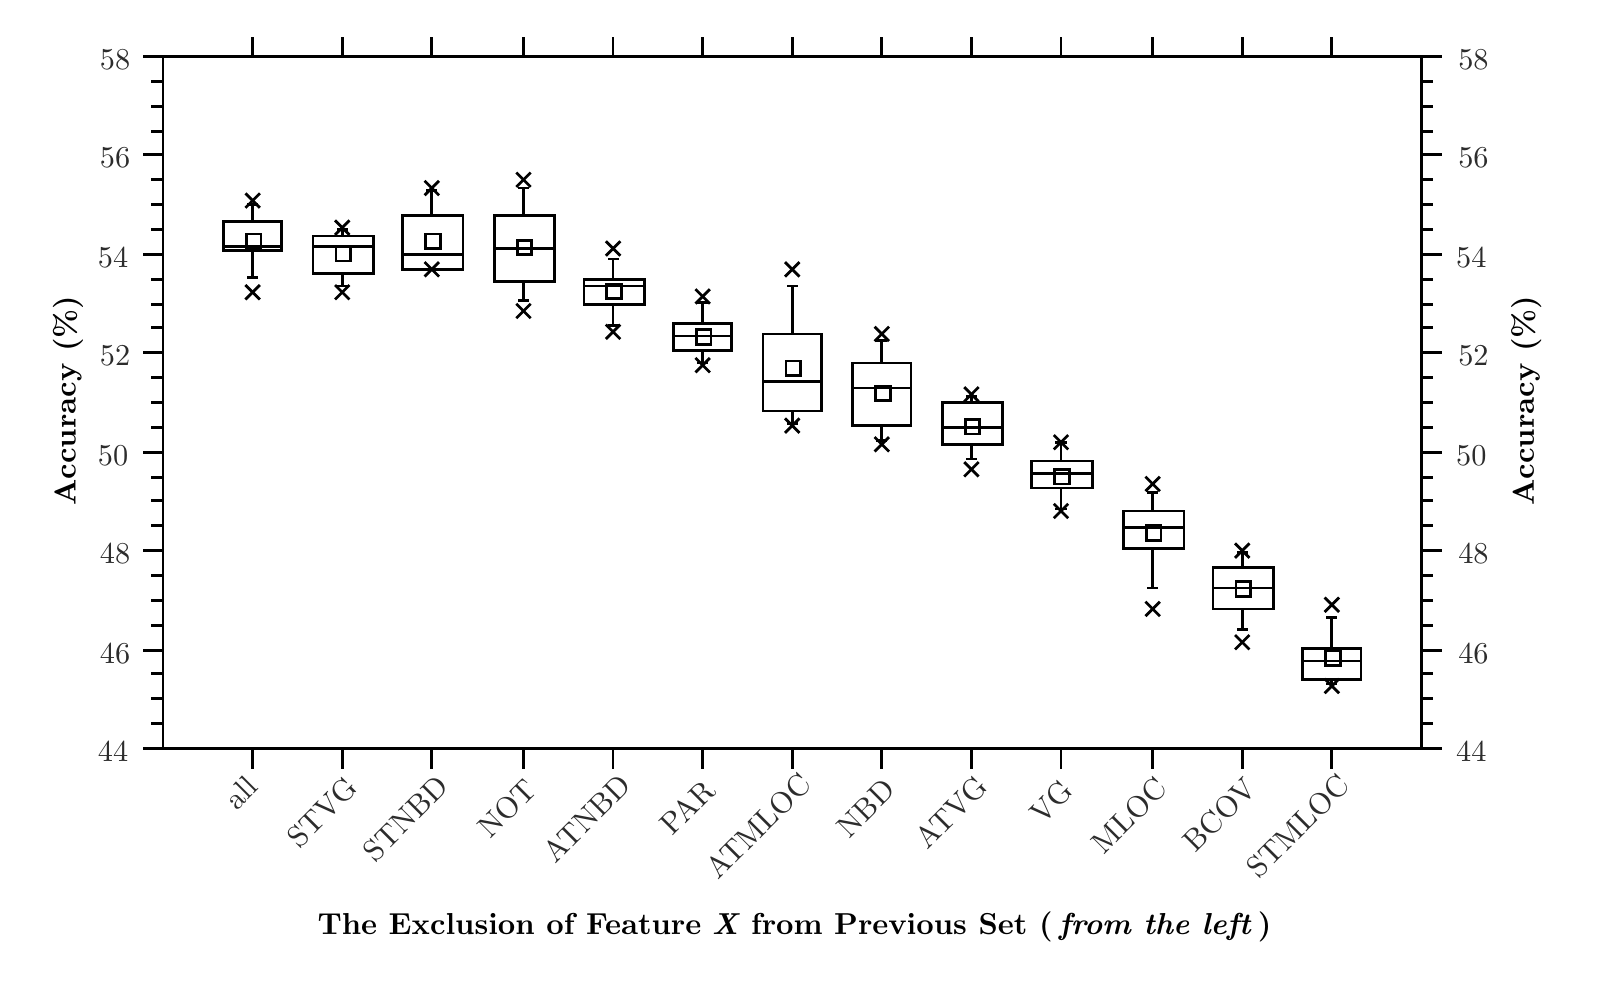
\begin{tikzpicture}{0pt}{0pt}{742pt}{452pt}
	\clip(0pt,452pt) -- (558.587pt,452pt) -- (558.587pt,111.729pt) -- (0pt,111.729pt) -- (0pt,452pt);
\begin{scope}
	\clip(48.9328pt,441.461pt) -- (503.632pt,441.461pt) -- (503.632pt,191.527pt) -- (48.9328pt,191.527pt) -- (48.9328pt,441.461pt);
	\color[rgb]{0,0,0}
	\draw[line width=1pt, line join=miter, line cap=rect](70.7644pt,381.988pt) -- (91.8431pt,381.988pt) -- (91.8431pt,371.449pt) -- (70.7644pt,371.449pt) -- (70.7644pt,381.988pt);
	\color[rgb]{0,0,0}
	\draw[line width=1pt, line join=miter, line cap=rect](79.7981pt,361.663pt) -- (82.8094pt,361.663pt);
	\draw[line width=1pt, line join=miter, line cap=rect](79.7981pt,388.011pt) -- (82.8094pt,388.011pt);
	\draw[line width=1pt, line join=miter, line cap=rect](81.3037pt,388.011pt) -- (81.3037pt,381.988pt);
	\draw[line width=1pt, line join=miter, line cap=rect](81.3037pt,361.663pt) -- (81.3037pt,371.449pt);
	\draw[line width=1pt, line join=miter, line cap=rect](70.7644pt,372.955pt) -- (91.8431pt,372.955pt);
	\draw[line width=1pt, line join=miter, line cap=rect](79.0453pt,358.651pt) -- (83.5622pt,354.134pt);
	\draw[line width=1pt, line join=miter, line cap=rect](79.0453pt,354.134pt) -- (83.5622pt,358.651pt);
	\draw[line width=1pt, line join=miter, line cap=rect](79.0453pt,391.775pt) -- (83.5622pt,387.258pt);
	\draw[line width=1pt, line join=miter, line cap=rect](79.0453pt,387.258pt) -- (83.5622pt,391.775pt);
	\draw[line width=1pt, line join=miter, line cap=rect](79.0453pt,377.472pt) -- (84.315pt,377.472pt) -- (84.315pt,372.202pt) -- (79.0453pt,372.202pt) -- (79.0453pt,377.472pt);
	\draw[line width=1pt, line join=miter, line cap=rect](103.135pt,376.719pt) -- (124.967pt,376.719pt) -- (124.967pt,363.168pt) -- (103.135pt,363.168pt) -- (103.135pt,376.719pt);
	\draw[line width=1pt, line join=miter, line cap=rect](112.169pt,358.651pt) -- (115.18pt,358.651pt);
	\draw[line width=1pt, line join=miter, line cap=rect](112.169pt,378.977pt) -- (115.18pt,378.977pt);
	\draw[line width=1pt, line join=miter, line cap=rect](113.675pt,378.977pt) -- (113.675pt,376.719pt);
	\draw[line width=1pt, line join=miter, line cap=rect](113.675pt,358.651pt) -- (113.675pt,363.168pt);
	\draw[line width=1pt, line join=miter, line cap=rect](103.135pt,372.955pt) -- (124.214pt,372.955pt);
	\draw[line width=1pt, line join=miter, line cap=rect](111.416pt,358.651pt) -- (115.933pt,354.134pt);
	\draw[line width=1pt, line join=miter, line cap=rect](111.416pt,354.134pt) -- (115.933pt,358.651pt);
	\draw[line width=1pt, line join=miter, line cap=rect](111.416pt,381.988pt) -- (115.933pt,377.472pt);
	\draw[line width=1pt, line join=miter, line cap=rect](111.416pt,377.472pt) -- (115.933pt,381.988pt);
	\draw[line width=1pt, line join=miter, line cap=rect](111.416pt,372.955pt) -- (116.686pt,372.955pt) -- (116.686pt,367.685pt) -- (111.416pt,367.685pt) -- (111.416pt,372.955pt);
	\draw[line width=1pt, line join=miter, line cap=rect](135.506pt,384.247pt) -- (157.338pt,384.247pt) -- (157.338pt,364.674pt) -- (135.506pt,364.674pt) -- (135.506pt,384.247pt);
	\draw[line width=1pt, line join=miter, line cap=rect](144.54pt,364.674pt) -- (147.551pt,364.674pt);
	\draw[line width=1pt, line join=miter, line cap=rect](144.54pt,393.281pt) -- (147.551pt,393.281pt);
	\draw[line width=1pt, line join=miter, line cap=rect](146.046pt,393.281pt) -- (146.046pt,384.247pt);

	\draw[line width=1pt, line join=miter, line cap=rect](135.506pt,369.943pt) -- (156.585pt,369.943pt);
	\draw[line width=1pt, line join=miter, line cap=rect](143.787pt,366.932pt) -- (148.304pt,362.415pt);
	\draw[line width=1pt, line join=miter, line cap=rect](143.787pt,362.415pt) -- (148.304pt,366.932pt);
	\draw[line width=1pt, line join=miter, line cap=rect](143.787pt,396.292pt) -- (148.304pt,391.775pt);
	\draw[line width=1pt, line join=miter, line cap=rect](143.787pt,391.775pt) -- (148.304pt,396.292pt);
	\draw[line width=1pt, line join=miter, line cap=rect](143.787pt,377.472pt) -- (149.057pt,377.472pt) -- (149.057pt,372.202pt) -- (143.787pt,372.202pt) -- (143.787pt,377.472pt);
	\draw[line width=1pt, line join=miter, line cap=rect](168.63pt,384.247pt) -- (190.462pt,384.247pt) -- (190.462pt,360.157pt) -- (168.63pt,360.157pt) -- (168.63pt,384.247pt);
	\draw[line width=1pt, line join=miter, line cap=rect](177.664pt,353.382pt) -- (180.675pt,353.382pt);
	\draw[line width=1pt, line join=miter, line cap=rect](177.664pt,394.033pt) -- (180.675pt,394.033pt);
	\draw[line width=1pt, line join=miter, line cap=rect](179.169pt,394.033pt) -- (179.169pt,384.247pt);
	\draw[line width=1pt, line join=miter, line cap=rect](179.169pt,353.382pt) -- (179.169pt,360.157pt);
	\draw[line width=1pt, line join=miter, line cap=rect](168.63pt,372.202pt) -- (189.709pt,372.202pt);
	\draw[line width=1pt, line join=miter, line cap=rect](176.911pt,351.876pt) -- (181.428pt,347.359pt);
	\draw[line width=1pt, line join=miter, line cap=rect](176.911pt,347.359pt) -- (181.428pt,351.876pt);
	\draw[line width=1pt, line join=miter, line cap=rect](176.911pt,399.303pt) -- (181.428pt,394.786pt);
	\draw[line width=1pt, line join=miter, line cap=rect](176.911pt,394.786pt) -- (181.428pt,399.303pt);
	\draw[line width=1pt, line join=miter, line cap=rect](176.911pt,375.213pt) -- (182.181pt,375.213pt) -- (182.181pt,369.943pt) -- (176.911pt,369.943pt) -- (176.911pt,375.213pt);
	\draw[line width=1pt, line join=miter, line cap=rect](201.001pt,360.91pt) -- (222.833pt,360.91pt) -- (222.833pt,351.876pt) -- (201.001pt,351.876pt) -- (201.001pt,360.91pt);
	\draw[line width=1pt, line join=miter, line cap=rect](210.035pt,344.348pt) -- (213.046pt,344.348pt);
	\draw[line width=1pt, line join=miter, line cap=rect](210.035pt,368.438pt) -- (213.046pt,368.438pt);
	\draw[line width=1pt, line join=miter, line cap=rect](211.54pt,368.438pt) -- (211.54pt,360.91pt);
	\draw[line width=1pt, line join=miter, line cap=rect](211.54pt,344.348pt) -- (211.54pt,351.876pt);
	\draw[line width=1pt, line join=miter, line cap=rect](201.001pt,358.651pt) -- (222.08pt,358.651pt);
	\draw[line width=1pt, line join=miter, line cap=rect](209.282pt,344.348pt) -- (213.799pt,339.831pt);
	\draw[line width=1pt, line join=miter, line cap=rect](209.282pt,339.831pt) -- (213.799pt,344.348pt);
	\draw[line width=1pt, line join=miter, line cap=rect](209.282pt,374.46pt) -- (213.799pt,369.943pt);
	\draw[line width=1pt, line join=miter, line cap=rect](209.282pt,369.943pt) -- (213.799pt,374.46pt);
	\draw[line width=1pt, line join=miter, line cap=rect](209.282pt,359.404pt) -- (214.552pt,359.404pt) -- (214.552pt,354.134pt) -- (209.282pt,354.134pt) -- (209.282pt,359.404pt);
	\draw[line width=1pt, line join=miter, line cap=rect](233.372pt,345.101pt) -- (254.451pt,345.101pt) -- (254.451pt,335.314pt) -- (233.372pt,335.314pt) -- (233.372pt,345.101pt);
	\draw[line width=1pt, line join=miter, line cap=rect](242.406pt,330.797pt) -- (245.417pt,330.797pt);
	\draw[line width=1pt, line join=miter, line cap=rect](242.406pt,352.629pt) -- (245.417pt,352.629pt);
	\draw[line width=1pt, line join=miter, line cap=rect](243.911pt,352.629pt) -- (243.911pt,345.101pt);
	\draw[line width=1pt, line join=miter, line cap=rect](243.911pt,330.797pt) -- (243.911pt,335.314pt);
	\draw[line width=1pt, line join=miter, line cap=rect](233.372pt,340.584pt) -- (254.451pt,340.584pt);
	\draw[line width=1pt, line join=miter, line cap=rect](241.653pt,332.303pt) -- (246.17pt,327.786pt);
	\draw[line width=1pt, line join=miter, line cap=rect](241.653pt,327.786pt) -- (246.17pt,332.303pt);
	\draw[line width=1pt, line join=miter, line cap=rect](241.653pt,357.146pt) -- (246.17pt,352.629pt);
	\draw[line width=1pt, line join=miter, line cap=rect](241.653pt,352.629pt) -- (246.17pt,357.146pt);
	\draw[line width=1pt, line join=miter, line cap=rect](241.653pt,342.842pt) -- (246.922pt,342.842pt) -- (246.922pt,337.572pt) -- (241.653pt,337.572pt) -- (241.653pt,342.842pt);
	\draw[line width=1pt, line join=miter, line cap=rect](265.743pt,341.337pt) -- (286.822pt,341.337pt) -- (286.822pt,313.482pt) -- (265.743pt,313.482pt) -- (265.743pt,341.337pt);
	\draw[line width=1pt, line join=miter, line cap=rect](274.777pt,308.966pt) -- (277.788pt,308.966pt);
	\draw[line width=1pt, line join=miter, line cap=rect](274.777pt,358.651pt) -- (277.788pt,358.651pt);
	\draw[line width=1pt, line join=miter, line cap=rect](276.282pt,358.651pt) -- (276.282pt,341.337pt);
	\draw[line width=1pt, line join=miter, line cap=rect](276.282pt,308.966pt) -- (276.282pt,313.482pt);
	\draw[line width=1pt, line join=miter, line cap=rect](265.743pt,324.022pt) -- (286.822pt,324.022pt);
	\draw[line width=1pt, line join=miter, line cap=rect](274.024pt,310.471pt) -- (278.541pt,305.954pt);
	\draw[line width=1pt, line join=miter, line cap=rect](274.024pt,305.954pt) -- (278.541pt,310.471pt);
	\draw[line width=1pt, line join=miter, line cap=rect](274.024pt,366.932pt) -- (278.541pt,362.415pt);
	\draw[line width=1pt, line join=miter, line cap=rect](274.024pt,362.415pt) -- (278.541pt,366.932pt);
	\draw[line width=1pt, line join=miter, line cap=rect](274.024pt,331.55pt) -- (279.293pt,331.55pt) -- (279.293pt,326.28pt) -- (274.024pt,326.28pt) -- (274.024pt,331.55pt);
	\draw[line width=1pt, line join=miter, line cap=rect](298.114pt,330.797pt) -- (319.192pt,330.797pt) -- (319.192pt,308.213pt) -- (298.114pt,308.213pt) -- (298.114pt,330.797pt);
	\draw[line width=1pt, line join=miter, line cap=rect](307.147pt,302.943pt) -- (310.159pt,302.943pt);
	\draw[line width=1pt, line join=miter, line cap=rect](307.147pt,339.078pt) -- (310.159pt,339.078pt);
	\draw[line width=1pt, line join=miter, line cap=rect](308.653pt,339.078pt) -- (308.653pt,330.797pt);
	\draw[line width=1pt, line join=miter, line cap=rect](308.653pt,302.943pt) -- (308.653pt,308.213pt);
	\draw[line width=1pt, line join=miter, line cap=rect](298.114pt,321.763pt) -- (319.192pt,321.763pt);
	\draw[line width=1pt, line join=miter, line cap=rect](306.395pt,303.696pt) -- (310.912pt,299.179pt);
	\draw[line width=1pt, line join=miter, line cap=rect](306.395pt,299.179pt) -- (310.912pt,303.696pt);
	\draw[line width=1pt, line join=miter, line cap=rect](306.395pt,343.595pt) -- (310.912pt,339.078pt);
	\draw[line width=1pt, line join=miter, line cap=rect](306.395pt,339.078pt) -- (310.912pt,343.595pt);
	\draw[line width=1pt, line join=miter, line cap=rect](306.395pt,322.516pt) -- (311.664pt,322.516pt) -- (311.664pt,317.247pt) -- (306.395pt,317.247pt) -- (306.395pt,322.516pt);
	\draw[line width=1pt, line join=miter, line cap=rect](330.485pt,316.494pt) -- (352.316pt,316.494pt) -- (352.316pt,301.438pt) -- (330.485pt,301.438pt) -- (330.485pt,316.494pt);
	\draw[line width=1pt, line join=miter, line cap=rect](339.518pt,296.168pt) -- (342.53pt,296.168pt);
	\draw[line width=1pt, line join=miter, line cap=rect](339.518pt,318.752pt) -- (342.53pt,318.752pt);
	\draw[line width=1pt, line join=miter, line cap=rect](341.024pt,318.752pt) -- (341.024pt,316.494pt);
	\draw[line width=1pt, line join=miter, line cap=rect](341.024pt,296.168pt) -- (341.024pt,301.438pt);
	\draw[line width=1pt, line join=miter, line cap=rect](330.485pt,307.46pt) -- (351.563pt,307.46pt);
	\draw[line width=1pt, line join=miter, line cap=rect](338.766pt,294.662pt) -- (343.282pt,290.145pt);
	\draw[line width=1pt, line join=miter, line cap=rect](338.766pt,290.145pt) -- (343.282pt,294.662pt);
	\draw[line width=1pt, line join=miter, line cap=rect](338.766pt,321.763pt) -- (343.282pt,317.247pt);
	\draw[line width=1pt, line join=miter, line cap=rect](338.766pt,317.247pt) -- (343.282pt,321.763pt);
	\draw[line width=1pt, line join=miter, line cap=rect](338.766pt,310.471pt) -- (344.035pt,310.471pt) -- (344.035pt,305.202pt) -- (338.766pt,305.202pt) -- (338.766pt,310.471pt);
	\draw[line width=1pt, line join=miter, line cap=rect](362.856pt,295.415pt) -- (384.687pt,295.415pt) -- (384.687pt,285.628pt) -- (362.856pt,285.628pt) -- (362.856pt,295.415pt);
	\draw[line width=1pt, line join=miter, line cap=rect](371.889pt,278.1pt) -- (374.901pt,278.1pt);
	\draw[line width=1pt, line join=miter, line cap=rect](371.889pt,302.19pt) -- (374.901pt,302.19pt);
	\draw[line width=1pt, line join=miter, line cap=rect](373.395pt,302.19pt) -- (373.395pt,295.415pt);
	\draw[line width=1pt, line join=miter, line cap=rect](373.395pt,278.1pt) -- (373.395pt,285.628pt);
	\draw[line width=1pt, line join=miter, line cap=rect](362.856pt,290.898pt) -- (383.934pt,290.898pt);
	\draw[line width=1pt, line join=miter, line cap=rect](371.137pt,279.606pt) -- (375.653pt,275.089pt);
	\draw[line width=1pt, line join=miter, line cap=rect](371.137pt,275.089pt) -- (375.653pt,279.606pt);
	\draw[line width=1pt, line join=miter, line cap=rect](371.137pt,304.449pt) -- (375.653pt,299.932pt);
	\draw[line width=1pt, line join=miter, line cap=rect](371.137pt,299.932pt) -- (375.653pt,304.449pt);
	\draw[line width=1pt, line join=miter, line cap=rect](371.137pt,292.404pt) -- (376.406pt,292.404pt) -- (376.406pt,287.134pt) -- (371.137pt,287.134pt) -- (371.137pt,292.404pt);
	\draw[line width=1pt, line join=miter, line cap=rect](395.979pt,277.347pt) -- (417.811pt,277.347pt) -- (417.811pt,263.797pt) -- (395.979pt,263.797pt) -- (395.979pt,277.347pt);
	\draw[line width=1pt, line join=miter, line cap=rect](405.013pt,249.493pt) -- (408.024pt,249.493pt);
	\draw[line width=1pt, line join=miter, line cap=rect](405.013pt,284.123pt) -- (408.024pt,284.123pt);
	\draw[line width=1pt, line join=miter, line cap=rect](406.519pt,284.123pt) -- (406.519pt,277.347pt);
	\draw[line width=1pt, line join=miter, line cap=rect](406.519pt,249.493pt) -- (406.519pt,263.797pt);
	\draw[line width=1pt, line join=miter, line cap=rect](395.979pt,271.325pt) -- (417.058pt,271.325pt);
	\draw[line width=1pt, line join=miter, line cap=rect](404.26pt,244.224pt) -- (408.777pt,239.707pt);
	\draw[line width=1pt, line join=miter, line cap=rect](404.26pt,239.707pt) -- (408.777pt,244.224pt);
	\draw[line width=1pt, line join=miter, line cap=rect](404.26pt,289.393pt) -- (408.777pt,284.876pt);
	\draw[line width=1pt, line join=miter, line cap=rect](404.26pt,284.876pt) -- (408.777pt,289.393pt);
	\draw[line width=1pt, line join=miter, line cap=rect](404.26pt,272.078pt) -- (409.53pt,272.078pt) -- (409.53pt,266.808pt) -- (404.26pt,266.808pt) -- (404.26pt,272.078pt);
	\draw[line width=1pt, line join=miter, line cap=rect](428.35pt,257.022pt) -- (450.182pt,257.022pt) -- (450.182pt,241.965pt) -- (428.35pt,241.965pt) -- (428.35pt,257.022pt);
	\draw[line width=1pt, line join=miter, line cap=rect](437.384pt,234.437pt) -- (440.395pt,234.437pt);
	\draw[line width=1pt, line join=miter, line cap=rect](437.384pt,262.291pt) -- (440.395pt,262.291pt);
	\draw[line width=1pt, line join=miter, line cap=rect](438.89pt,262.291pt) -- (438.89pt,257.022pt);
	\draw[line width=1pt, line join=miter, line cap=rect](438.89pt,234.437pt) -- (438.89pt,241.965pt);
	\draw[line width=1pt, line join=miter, line cap=rect](428.35pt,249.493pt) -- (449.429pt,249.493pt);
	\draw[line width=1pt, line join=miter, line cap=rect](436.631pt,232.179pt) -- (441.148pt,227.662pt);
	\draw[line width=1pt, line join=miter, line cap=rect](436.631pt,227.662pt) -- (441.148pt,232.179pt);
	\draw[line width=1pt, line join=miter, line cap=rect](436.631pt,265.303pt) -- (441.148pt,260.786pt);
	\draw[line width=1pt, line join=miter, line cap=rect](436.631pt,260.786pt) -- (441.148pt,265.303pt);
	\draw[line width=1pt, line join=miter, line cap=rect](436.631pt,251.752pt) -- (441.901pt,251.752pt) -- (441.901pt,246.482pt) -- (436.631pt,246.482pt) -- (436.631pt,251.752pt);
	\draw[line width=1pt, line join=miter, line cap=rect](460.721pt,227.662pt) -- (481.8pt,227.662pt) -- (481.8pt,216.37pt) -- (460.721pt,216.37pt) -- (460.721pt,227.662pt);
	\draw[line width=1pt, line join=miter, line cap=rect](469.755pt,214.864pt) -- (472.766pt,214.864pt);
	\draw[line width=1pt, line join=miter, line cap=rect](469.755pt,238.954pt) -- (472.766pt,238.954pt);
	\draw[line width=1pt, line join=miter, line cap=rect](471.261pt,238.954pt) -- (471.261pt,227.662pt);
	\draw[line width=1pt, line join=miter, line cap=rect](471.261pt,214.864pt) -- (471.261pt,216.37pt);
	\draw[line width=1pt, line join=miter, line cap=rect](460.721pt,223.145pt) -- (481.8pt,223.145pt);
	\draw[line width=1pt, line join=miter, line cap=rect](469.002pt,216.37pt) -- (473.519pt,211.853pt);
	\draw[line width=1pt, line join=miter, line cap=rect](469.002pt,211.853pt) -- (473.519pt,216.37pt);
	\draw[line width=1pt, line join=miter, line cap=rect](469.002pt,245.729pt) -- (473.519pt,241.213pt);
	\draw[line width=1pt, line join=miter, line cap=rect](469.002pt,241.213pt) -- (473.519pt,245.729pt);
	\draw[line width=1pt, line join=miter, line cap=rect](469.002pt,226.909pt) -- (474.272pt,226.909pt) -- (474.272pt,221.639pt) -- (469.002pt,221.639pt) -- (469.002pt,226.909pt);
\end{scope}
\begin{scope}
	\color[rgb]{0,0,0}
	\pgftext[center, base, at={\pgfpoint{17.3147pt}{317.247pt}},rotate=90]{\fontsize{11}{0}\selectfont{\textbf{Accuracy (\%)}}}
	\color[rgb]{0.172549,0.172549,0.172549}
	\pgftext[center, base, at={\pgfpoint{30.8535pt}{187.01pt}}]{\fontsize{11}{0}\selectfont{44}}
	\pgftext[center, base, at={\pgfpoint{31.6064pt}{222.392pt}}]{\fontsize{11}{0}\selectfont{46}}
	\pgftext[center, base, at={\pgfpoint{31.6064pt}{258.527pt}}]{\fontsize{11}{0}\selectfont{48}}
	\pgftext[center, base, at={\pgfpoint{30.8535pt}{293.909pt}}]{\fontsize{11}{0}\selectfont{50}}
	\pgftext[center, base, at={\pgfpoint{31.6064pt}{330.044pt}}]{\fontsize{11}{0}\selectfont{52}}
	\pgftext[center, base, at={\pgfpoint{30.8535pt}{365.427pt}}]{\fontsize{11}{0}\selectfont{54}}
	\pgftext[center, base, at={\pgfpoint{31.6064pt}{401.562pt}}]{\fontsize{11}{0}\selectfont{56}}
	\pgftext[center, base, at={\pgfpoint{31.6064pt}{436.944pt}}]{\fontsize{11}{0}\selectfont{58}}
	\color[rgb]{0,0,0}
	\draw[line width=1pt, line join=bevel, line cap=rect](48.9328pt,200.561pt) -- (45.1688pt,200.561pt);
	\draw[line width=1pt, line join=bevel, line cap=rect](48.9328pt,218.628pt) -- (45.1688pt,218.628pt);
	\draw[line width=1pt, line join=bevel, line cap=rect](48.9328pt,235.943pt) -- (45.1688pt,235.943pt);
	\draw[line width=1pt, line join=bevel, line cap=rect](48.9328pt,254.01pt) -- (45.1688pt,254.01pt);
	\draw[line width=1pt, line join=bevel, line cap=rect](48.9328pt,272.078pt) -- (45.1688pt,272.078pt);
	\draw[line width=1pt, line join=bevel, line cap=rect](48.9328pt,289.393pt) -- (45.1688pt,289.393pt);
	\draw[line width=1pt, line join=bevel, line cap=rect](48.9328pt,307.46pt) -- (45.1688pt,307.46pt);
	\draw[line width=1pt, line join=bevel, line cap=rect](48.9328pt,325.528pt) -- (45.1688pt,325.528pt);
	\draw[line width=1pt, line join=bevel, line cap=rect](48.9328pt,343.595pt) -- (45.1688pt,343.595pt);
	\draw[line width=1pt, line join=bevel, line cap=rect](48.9328pt,360.91pt) -- (45.1688pt,360.91pt);
	\draw[line width=1pt, line join=bevel, line cap=rect](48.9328pt,378.977pt) -- (45.1688pt,378.977pt);
	\draw[line width=1pt, line join=bevel, line cap=rect](48.9328pt,397.045pt) -- (45.1688pt,397.045pt);
	\draw[line width=1pt, line join=bevel, line cap=rect](48.9328pt,414.359pt) -- (45.1688pt,414.359pt);
	\draw[line width=1pt, line join=bevel, line cap=rect](48.9328pt,432.427pt) -- (45.1688pt,432.427pt);
	\draw[line width=1pt, line join=bevel, line cap=rect](48.9328pt,209.594pt) -- (45.1688pt,209.594pt);
	\draw[line width=1pt, line join=bevel, line cap=rect](48.9328pt,244.977pt) -- (45.1688pt,244.977pt);
	\draw[line width=1pt, line join=bevel, line cap=rect](48.9328pt,281.112pt) -- (45.1688pt,281.112pt);
	\draw[line width=1pt, line join=bevel, line cap=rect](48.9328pt,316.494pt) -- (45.1688pt,316.494pt);
	\draw[line width=1pt, line join=bevel, line cap=rect](48.9328pt,351.876pt) -- (45.1688pt,351.876pt);
	\draw[line width=1pt, line join=bevel, line cap=rect](48.9328pt,388.011pt) -- (45.1688pt,388.011pt);
	\draw[line width=1pt, line join=bevel, line cap=rect](48.9328pt,423.393pt) -- (45.1688pt,423.393pt);
	\draw[line width=1pt, line join=bevel, line cap=rect](48.9328pt,191.527pt) -- (42.1575pt,191.527pt);
	\draw[line width=1pt, line join=bevel, line cap=rect](48.9328pt,226.909pt) -- (42.1575pt,226.909pt);
	\draw[line width=1pt, line join=bevel, line cap=rect](48.9328pt,263.044pt) -- (42.1575pt,263.044pt);
	\draw[line width=1pt, line join=bevel, line cap=rect](48.9328pt,298.426pt) -- (42.1575pt,298.426pt);
	\draw[line width=1pt, line join=bevel, line cap=rect](48.9328pt,334.561pt) -- (42.1575pt,334.561pt);
	\draw[line width=1pt, line join=bevel, line cap=rect](48.9328pt,369.943pt) -- (42.1575pt,369.943pt);
	\draw[line width=1pt, line join=bevel, line cap=rect](48.9328pt,406.078pt) -- (42.1575pt,406.078pt);
	\draw[line width=1pt, line join=bevel, line cap=rect](48.9328pt,441.461pt) -- (42.1575pt,441.461pt);
	\draw[line width=1pt, line join=bevel, line cap=rect](48.9328pt,441.461pt) -- (48.9328pt,191.527pt);
	\pgftext[center, base, at={\pgfpoint{544.283pt}{317.247pt}},rotate=90]{\fontsize{11}{0}\selectfont{\textbf{Accuracy (\%)}}}
	\color[rgb]{0.172549,0.172549,0.172549}
	\pgftext[center, base, at={\pgfpoint{521.687pt}{187.01pt}}]{\fontsize{11}{0}\selectfont{44}}
	\pgftext[center, base, at={\pgfpoint{522.44pt}{222.392pt}}]{\fontsize{11}{0}\selectfont{46}}
	\pgftext[center, base, at={\pgfpoint{522.44pt}{258.527pt}}]{\fontsize{11}{0}\selectfont{48}}
	\pgftext[center, base, at={\pgfpoint{521.687pt}{293.909pt}}]{\fontsize{11}{0}\selectfont{50}}
	\pgftext[center, base, at={\pgfpoint{522.44pt}{330.044pt}}]{\fontsize{11}{0}\selectfont{52}}
	\pgftext[center, base, at={\pgfpoint{521.687pt}{365.427pt}}]{\fontsize{11}{0}\selectfont{54}}
	\pgftext[center, base, at={\pgfpoint{522.44pt}{401.562pt}}]{\fontsize{11}{0}\selectfont{56}}
	\pgftext[center, base, at={\pgfpoint{522.44pt}{436.944pt}}]{\fontsize{11}{0}\selectfont{58}}
	\color[rgb]{0,0,0}
	\draw[line width=1pt, line join=bevel, line cap=rect](503.632pt,200.561pt) -- (507.396pt,200.561pt);
	\draw[line width=1pt, line join=bevel, line cap=rect](503.632pt,218.628pt) -- (507.396pt,218.628pt);
	\draw[line width=1pt, line join=bevel, line cap=rect](503.632pt,235.943pt) -- (507.396pt,235.943pt);
	\draw[line width=1pt, line join=bevel, line cap=rect](503.632pt,254.01pt) -- (507.396pt,254.01pt);
	\draw[line width=1pt, line join=bevel, line cap=rect](503.632pt,272.078pt) -- (507.396pt,272.078pt);
	\draw[line width=1pt, line join=bevel, line cap=rect](503.632pt,289.393pt) -- (507.396pt,289.393pt);
	\draw[line width=1pt, line join=bevel, line cap=rect](503.632pt,307.46pt) -- (507.396pt,307.46pt);
	\draw[line width=1pt, line join=bevel, line cap=rect](503.632pt,325.528pt) -- (507.396pt,325.528pt);
	\draw[line width=1pt, line join=bevel, line cap=rect](503.632pt,343.595pt) -- (507.396pt,343.595pt);
	\draw[line width=1pt, line join=bevel, line cap=rect](503.632pt,360.91pt) -- (507.396pt,360.91pt);
	\draw[line width=1pt, line join=bevel, line cap=rect](503.632pt,378.977pt) -- (507.396pt,378.977pt);
	\draw[line width=1pt, line join=bevel, line cap=rect](503.632pt,397.045pt) -- (507.396pt,397.045pt);
	\draw[line width=1pt, line join=bevel, line cap=rect](503.632pt,414.359pt) -- (507.396pt,414.359pt);
	\draw[line width=1pt, line join=bevel, line cap=rect](503.632pt,432.427pt) -- (507.396pt,432.427pt);
	\draw[line width=1pt, line join=bevel, line cap=rect](503.632pt,209.594pt) -- (507.396pt,209.594pt);
	\draw[line width=1pt, line join=bevel, line cap=rect](503.632pt,244.977pt) -- (507.396pt,244.977pt);
	\draw[line width=1pt, line join=bevel, line cap=rect](503.632pt,281.112pt) -- (507.396pt,281.112pt);
	\draw[line width=1pt, line join=bevel, line cap=rect](503.632pt,316.494pt) -- (507.396pt,316.494pt);
	\draw[line width=1pt, line join=bevel, line cap=rect](503.632pt,351.876pt) -- (507.396pt,351.876pt);
	\draw[line width=1pt, line join=bevel, line cap=rect](503.632pt,388.011pt) -- (507.396pt,388.011pt);
	\draw[line width=1pt, line join=bevel, line cap=rect](503.632pt,423.393pt) -- (507.396pt,423.393pt);
	\draw[line width=1pt, line join=bevel, line cap=rect](503.632pt,191.527pt) -- (510.407pt,191.527pt);
	\draw[line width=1pt, line join=bevel, line cap=rect](503.632pt,226.909pt) -- (510.407pt,226.909pt);
	\draw[line width=1pt, line join=bevel, line cap=rect](503.632pt,263.044pt) -- (510.407pt,263.044pt);
	\draw[line width=1pt, line join=bevel, line cap=rect](503.632pt,298.426pt) -- (510.407pt,298.426pt);
	\draw[line width=1pt, line join=bevel, line cap=rect](503.632pt,334.561pt) -- (510.407pt,334.561pt);
	\draw[line width=1pt, line join=bevel, line cap=rect](503.632pt,369.943pt) -- (510.407pt,369.943pt);
	\draw[line width=1pt, line join=bevel, line cap=rect](503.632pt,406.078pt) -- (510.407pt,406.078pt);
	\draw[line width=1pt, line join=bevel, line cap=rect](503.632pt,441.461pt) -- (510.407pt,441.461pt);
	\draw[line width=1pt, line join=bevel, line cap=rect](503.632pt,441.461pt) -- (503.632pt,191.527pt);
	\pgftext[center, base, at={\pgfpoint{176.17pt}{124.291pt}}]{\fontsize{11}{0}\selectfont{\textbf{The Exclusion of Feature }}}
	\pgftext[center, base, at={\pgfpoint{252.839pt}{124.291pt}}]{\fontsize{11}{0}\selectfont{\textit{\textbf{X}}}}
	\pgftext[center, base, at={\pgfpoint{313.788pt}{124.291pt}}]{\fontsize{11}{0}\selectfont{\textbf{ from Previous Set (}}}
	\pgftext[center, base, at={\pgfpoint{407.777pt}{124.291pt}}]{\fontsize{11}{0}\selectfont{\textit{\textbf{from the left}}}}
	\pgftext[center, base, at={\pgfpoint{446.941pt}{124.291pt}}]{\fontsize{11}{0}\selectfont{\textbf{)}}}
	\color[rgb]{0.172549,0.172549,0.172549}
	\pgftext[center, base, at={\pgfpoint{79.5529pt}{172.849pt}},rotate=45]{\fontsize{11}{0}\selectfont{all}}
	\pgftext[center, base, at={\pgfpoint{108.938pt}{165.863pt}},rotate=45]{\fontsize{11}{0}\selectfont{STVG}}
	\pgftext[center, base, at={\pgfpoint{139.096pt}{163.65pt}},rotate=45]{\fontsize{11}{0}\selectfont{STNBD}}
	\pgftext[center, base, at={\pgfpoint{175.776pt}{167.206pt}},rotate=45]{\fontsize{11}{0}\selectfont{NOT}}
	\pgftext[center, base, at={\pgfpoint{204.566pt}{163.625pt}},rotate=45]{\fontsize{11}{0}\selectfont{ATNBD}}
	\pgftext[center, base, at={\pgfpoint{240.942pt}{167.63pt}},rotate=45]{\fontsize{11}{0}\selectfont{PAR}}
	\pgftext[center, base, at={\pgfpoint{266.526pt}{160.843pt}},rotate=45]{\fontsize{11}{0}\selectfont{ATMLOC}}
	\pgftext[center, base, at={\pgfpoint{305.451pt}{167.397pt}},rotate=45]{\fontsize{11}{0}\selectfont{NBD}}
	\pgftext[center, base, at={\pgfpoint{336.262pt}{165.838pt}},rotate=45]{\fontsize{11}{0}\selectfont{ATVG}}
	\pgftext[center, base, at={\pgfpoint{372.405pt}{169.61pt}},rotate=45]{\fontsize{11}{0}\selectfont{VG}}
	\pgftext[center, base, at={\pgfpoint{400.534pt}{164.615pt}},rotate=45]{\fontsize{11}{0}\selectfont{MLOC}}
	\pgftext[center, base, at={\pgfpoint{433.242pt}{164.952pt}},rotate=45]{\fontsize{11}{0}\selectfont{BCOV}}
	\pgftext[center, base, at={\pgfpoint{461.529pt}{160.868pt}},rotate=45]{\fontsize{11}{0}\selectfont{STMLOC}}
	\color[rgb]{0,0,0}
	\draw[line width=1pt, line join=bevel, line cap=rect](81.3037pt,191.527pt) -- (81.3037pt,184.752pt);
	\draw[line width=1pt, line join=bevel, line cap=rect](113.675pt,191.527pt) -- (113.675pt,184.752pt);
	\draw[line width=1pt, line join=bevel, line cap=rect](146.046pt,191.527pt) -- (146.046pt,184.752pt);
	\draw[line width=1pt, line join=bevel, line cap=rect](179.169pt,191.527pt) -- (179.169pt,184.752pt);
	\draw[line width=1pt, line join=bevel, line cap=rect](211.54pt,191.527pt) -- (211.54pt,184.752pt);
	\draw[line width=1pt, line join=bevel, line cap=rect](243.911pt,191.527pt) -- (243.911pt,184.752pt);
	\draw[line width=1pt, line join=bevel, line cap=rect](276.282pt,191.527pt) -- (276.282pt,184.752pt);
	\draw[line width=1pt, line join=bevel, line cap=rect](308.653pt,191.527pt) -- (308.653pt,184.752pt);
	\draw[line width=1pt, line join=bevel, line cap=rect](341.024pt,191.527pt) -- (341.024pt,184.752pt);
	\draw[line width=1pt, line join=bevel, line cap=rect](373.395pt,191.527pt) -- (373.395pt,184.752pt);
	\draw[line width=1pt, line join=bevel, line cap=rect](406.519pt,191.527pt) -- (406.519pt,184.752pt);
	\draw[line width=1pt, line join=bevel, line cap=rect](438.89pt,191.527pt) -- (438.89pt,184.752pt);
	\draw[line width=1pt, line join=bevel, line cap=rect](471.261pt,191.527pt) -- (471.261pt,184.752pt);
	\draw[line width=1pt, line join=bevel, line cap=rect](48.9328pt,191.527pt) -- (503.632pt,191.527pt);
	\draw[line width=1pt, line join=bevel, line cap=rect](81.3037pt,441.461pt) -- (81.3037pt,448.236pt);
	\draw[line width=1pt, line join=bevel, line cap=rect](113.675pt,441.461pt) -- (113.675pt,448.236pt);
	\draw[line width=1pt, line join=bevel, line cap=rect](146.046pt,441.461pt) -- (146.046pt,448.236pt);
	\draw[line width=1pt, line join=bevel, line cap=rect](179.169pt,441.461pt) -- (179.169pt,448.236pt);
	\draw[line width=1pt, line join=bevel, line cap=rect](211.54pt,441.461pt) -- (211.54pt,448.236pt);
	\draw[line width=1pt, line join=bevel, line cap=rect](243.911pt,441.461pt) -- (243.911pt,448.236pt);
	\draw[line width=1pt, line join=bevel, line cap=rect](276.282pt,441.461pt) -- (276.282pt,448.236pt);
	\draw[line width=1pt, line join=bevel, line cap=rect](308.653pt,441.461pt) -- (308.653pt,448.236pt);
	\draw[line width=1pt, line join=bevel, line cap=rect](341.024pt,441.461pt) -- (341.024pt,448.236pt);
	\draw[line width=1pt, line join=bevel, line cap=rect](373.395pt,441.461pt) -- (373.395pt,448.236pt);
	\draw[line width=1pt, line join=bevel, line cap=rect](406.519pt,441.461pt) -- (406.519pt,448.236pt);
	\draw[line width=1pt, line join=bevel, line cap=rect](438.89pt,441.461pt) -- (438.89pt,448.236pt);
	\draw[line width=1pt, line join=bevel, line cap=rect](471.261pt,441.461pt) -- (471.261pt,448.236pt);
	\draw[line width=1pt, line join=bevel, line cap=rect](48.9328pt,441.461pt) -- (503.632pt,441.461pt);
\end{scope}
\end{tikzpicture}

  \end{adjustbox}
  \caption{Method-level cross-validation accuracy on the \emph{all} subject over an iterative exclusion of features}
  \vspace{1mm}
  \footnotesize{\emph{The last feature not removed is `BTOT'.}}
  \vspace{2mm}
  \hrule
  \label{fig:cross_validation_feature_selection_method_graph}
\end{figure}

The class-level cross-validation accuracy of the iteratively excluded features is shown in Figure~\ref{fig:cross_validation_feature_selection_class_graph}. We can see an interesting trend from the iterative exclusion of features, there is variation yet the mean accuracy remains approximately the same for about 17 iterations. After 17 iterations the cross-validation accuracy drops, which suggests that it is possible to exclude 17 features and still have approximately the same mean accuracy as with all the features. With respect to feature selection, an ideal situation would allow use to use a reduced set of features that actually increase the cross-validation accuracy (i.e., by removing detrimental features). In our case we did not see any substantial increase in cross-validation accuracy, though we did not lower the mean accuracy over 17 iterations of exclusions. Another ideal situation is to completely remove certain feature sets, thus freeing us from the collection of these features. We can completely remove the coverage metrics (feature set \ding{173}) as all those metrics are excluded through the iterations. We need to keep in mind that \gls{cfs} is a filter that removes features based on correlation with the category yet not with each other. An excluded feature might not necessarily be a \emph{bad} feature, it might just be redundant. In the case of class-level features we can see that \emph{STNBD} and \emph{STVG} are the first two features excluded using \gls{cfs} which makes sense considering both their correlation with the second last feature excluded (\emph{STMLOC}) is above 0.995. One interesting note here is that the last three features are each from three different feature sets (\emph{STMLOC} belongs to \ding{175}, \emph{SMLOC} belongs to \ding{174} and \emph{NOF} belongs to \ding{172}), which reinforces that each feature set is crucial to prediction and that the other features within these sets might be redundant.

The method-level cross-validation accuracy of iteratively excluding features (see Figure~\ref{fig:cross_validation_feature_selection_method_graph}) follows a similar trend to that of the class-level. If we consider the same approach as in the class-level we could potentially remove the first three features, which maintains the mean accuracy with a lesser amount of features. Unfortunately, it is not possible to completely remove a feature set with the exclusion of the first three features. Also we can see a similar trend in the order of excluded features that \emph{STVG}, \emph{STNBD} and \emph{NOT} are removed early on with \emph{STMLOC} and \emph{MLOC} (i.e., similar to \emph{SMLOC} from the class-level) being the last ones removed again due to high correlation between these features. The last four features for method-level contain one feature from each feature set (i.e., the applicable ones for method-level, which excludes \ding{174}), which again reinforces the necessity of these feature sets.

\begin{figure}[ht!]
  \centering
  \begin{adjustbox}{max size={.95\textwidth}{.95\textheight}}
    \begin{tikzpicture}{0pt}{0pt}{742pt}{452pt}
	\clip(0pt,452pt) -- (558.587pt,452pt) -- (558.587pt,111.729pt) -- (0pt,111.729pt) -- (0pt,452pt);
\begin{scope}
	\clip(58.7194pt,439.955pt) -- (499.115pt,439.955pt) -- (499.115pt,162.167pt) -- (58.7194pt,162.167pt) -- (58.7194pt,439.955pt);
	\color[rgb]{0,0,0}
	\draw[line width=1pt, line join=miter, line cap=rect](158.843pt,343.595pt) -- (252.945pt,343.595pt) -- (252.945pt,317.999pt) -- (158.843pt,317.999pt) -- (158.843pt,343.595pt);
	\color[rgb]{0,0,0}
	\draw[line width=1pt, line join=miter, line cap=rect](196.484pt,306.707pt) -- (214.552pt,306.707pt);
	\draw[line width=1pt, line join=miter, line cap=rect](196.484pt,372.955pt) -- (214.552pt,372.955pt);
	\draw[line width=1pt, line join=miter, line cap=rect](205.518pt,372.955pt) -- (205.518pt,343.595pt);
	\draw[line width=1pt, line join=miter, line cap=rect](205.518pt,306.707pt) -- (205.518pt,317.999pt);
	\draw[line width=1pt, line join=miter, line cap=rect](158.843pt,328.539pt) -- (252.192pt,328.539pt);
	\draw[line width=1pt, line join=miter, line cap=rect](203.259pt,295.415pt) -- (207.776pt,290.898pt);
	\draw[line width=1pt, line join=miter, line cap=rect](203.259pt,290.898pt) -- (207.776pt,295.415pt);
	\draw[line width=1pt, line join=miter, line cap=rect](203.259pt,399.303pt) -- (207.776pt,394.786pt);
	\draw[line width=1pt, line join=miter, line cap=rect](203.259pt,394.786pt) -- (207.776pt,399.303pt);
	\draw[line width=1pt, line join=miter, line cap=rect](203.259pt,333.808pt) -- (208.529pt,333.808pt) -- (208.529pt,328.539pt) -- (203.259pt,328.539pt) -- (203.259pt,333.808pt);
	\draw[line width=1pt, line join=miter, line cap=rect](305.642pt,230.673pt) -- (399.743pt,230.673pt) -- (399.743pt,204.325pt) -- (305.642pt,204.325pt) -- (305.642pt,230.673pt);
	\draw[line width=1pt, line join=miter, line cap=rect](343.282pt,196.797pt) -- (361.35pt,196.797pt);
	\draw[line width=1pt, line join=miter, line cap=rect](343.282pt,255.516pt) -- (361.35pt,255.516pt);
	\draw[line width=1pt, line join=miter, line cap=rect](352.316pt,255.516pt) -- (352.316pt,230.673pt);
	\draw[line width=1pt, line join=miter, line cap=rect](352.316pt,196.797pt) -- (352.316pt,204.325pt);
	\draw[line width=1pt, line join=miter, line cap=rect](305.642pt,217.123pt) -- (398.991pt,217.123pt);
	\draw[line width=1pt, line join=miter, line cap=rect](350.058pt,189.268pt) -- (354.575pt,184.752pt);
	\draw[line width=1pt, line join=miter, line cap=rect](350.058pt,184.752pt) -- (354.575pt,189.268pt);
	\draw[line width=1pt, line join=miter, line cap=rect](350.058pt,296.168pt) -- (354.575pt,291.651pt);
	\draw[line width=1pt, line join=miter, line cap=rect](350.058pt,291.651pt) -- (354.575pt,296.168pt);
	\draw[line width=1pt, line join=miter, line cap=rect](350.058pt,221.639pt) -- (355.327pt,221.639pt) -- (355.327pt,216.37pt) -- (350.058pt,216.37pt) -- (350.058pt,221.639pt);
\end{scope}
\begin{scope}
	\color[rgb]{0,0,0}
	\pgftext[center, base, at={\pgfpoint{17.3147pt}{301.814pt}},rotate=90]{\fontsize{11}{0}\selectfont{\textbf{Time (seconds)}}}
	\color[rgb]{0.172549,0.172549,0.172549}
	\pgftext[center, base, at={\pgfpoint{35.7939pt}{157.65pt}}]{\fontsize{11}{0}\selectfont{0.14}}
	\pgftext[center, base, at={\pgfpoint{35.7939pt}{197.549pt}}]{\fontsize{11}{0}\selectfont{0.16}}
	\pgftext[center, base, at={\pgfpoint{35.7939pt}{236.696pt}}]{\fontsize{11}{0}\selectfont{0.18}}
	\pgftext[center, base, at={\pgfpoint{39.6991pt}{276.595pt}}]{\fontsize{11}{0}\selectfont{0.2}}
	\pgftext[center, base, at={\pgfpoint{35.7939pt}{316.494pt}}]{\fontsize{11}{0}\selectfont{0.22}}
	\pgftext[center, base, at={\pgfpoint{35.7939pt}{356.393pt}}]{\fontsize{11}{0}\selectfont{0.24}}
	\pgftext[center, base, at={\pgfpoint{35.7939pt}{395.539pt}}]{\fontsize{11}{0}\selectfont{0.26}}
	\pgftext[center, base, at={\pgfpoint{35.7939pt}{435.438pt}}]{\fontsize{11}{0}\selectfont{0.28}}
	\color[rgb]{0,0,0}
	\draw[line width=1pt, line join=bevel, line cap=rect](58.7194pt,171.954pt) -- (54.9553pt,171.954pt);
	\draw[line width=1pt, line join=bevel, line cap=rect](58.7194pt,192.28pt) -- (54.9553pt,192.28pt);
	\draw[line width=1pt, line join=bevel, line cap=rect](58.7194pt,211.853pt) -- (54.9553pt,211.853pt);
	\draw[line width=1pt, line join=bevel, line cap=rect](58.7194pt,231.426pt) -- (54.9553pt,231.426pt);
	\draw[line width=1pt, line join=bevel, line cap=rect](58.7194pt,251.752pt) -- (54.9553pt,251.752pt);
	\draw[line width=1pt, line join=bevel, line cap=rect](58.7194pt,271.325pt) -- (54.9553pt,271.325pt);
	\draw[line width=1pt, line join=bevel, line cap=rect](58.7194pt,290.898pt) -- (54.9553pt,290.898pt);
	\draw[line width=1pt, line join=bevel, line cap=rect](58.7194pt,311.224pt) -- (54.9553pt,311.224pt);
	\draw[line width=1pt, line join=bevel, line cap=rect](58.7194pt,330.797pt) -- (54.9553pt,330.797pt);
	\draw[line width=1pt, line join=bevel, line cap=rect](58.7194pt,350.37pt) -- (54.9553pt,350.37pt);
	\draw[line width=1pt, line join=bevel, line cap=rect](58.7194pt,370.696pt) -- (54.9553pt,370.696pt);
	\draw[line width=1pt, line join=bevel, line cap=rect](58.7194pt,390.269pt) -- (54.9553pt,390.269pt);
	\draw[line width=1pt, line join=bevel, line cap=rect](58.7194pt,409.842pt) -- (54.9553pt,409.842pt);
	\draw[line width=1pt, line join=bevel, line cap=rect](58.7194pt,430.168pt) -- (54.9553pt,430.168pt);
	\draw[line width=1pt, line join=bevel, line cap=rect](58.7194pt,181.74pt) -- (54.9553pt,181.74pt);
	\draw[line width=1pt, line join=bevel, line cap=rect](58.7194pt,221.639pt) -- (54.9553pt,221.639pt);
	\draw[line width=1pt, line join=bevel, line cap=rect](58.7194pt,261.538pt) -- (54.9553pt,261.538pt);
	\draw[line width=1pt, line join=bevel, line cap=rect](58.7194pt,300.685pt) -- (54.9553pt,300.685pt);
	\draw[line width=1pt, line join=bevel, line cap=rect](58.7194pt,340.584pt) -- (54.9553pt,340.584pt);
	\draw[line width=1pt, line join=bevel, line cap=rect](58.7194pt,380.483pt) -- (54.9553pt,380.483pt);
	\draw[line width=1pt, line join=bevel, line cap=rect](58.7194pt,420.382pt) -- (54.9553pt,420.382pt);
	\draw[line width=1pt, line join=bevel, line cap=rect](58.7194pt,162.167pt) -- (51.9441pt,162.167pt);
	\draw[line width=1pt, line join=bevel, line cap=rect](58.7194pt,202.066pt) -- (51.9441pt,202.066pt);
	\draw[line width=1pt, line join=bevel, line cap=rect](58.7194pt,241.213pt) -- (51.9441pt,241.213pt);
	\draw[line width=1pt, line join=bevel, line cap=rect](58.7194pt,281.112pt) -- (51.9441pt,281.112pt);
	\draw[line width=1pt, line join=bevel, line cap=rect](58.7194pt,321.011pt) -- (51.9441pt,321.011pt);
	\draw[line width=1pt, line join=bevel, line cap=rect](58.7194pt,360.91pt) -- (51.9441pt,360.91pt);
	\draw[line width=1pt, line join=bevel, line cap=rect](58.7194pt,400.056pt) -- (51.9441pt,400.056pt);
	\draw[line width=1pt, line join=bevel, line cap=rect](58.7194pt,439.955pt) -- (51.9441pt,439.955pt);
	\draw[line width=1pt, line join=bevel, line cap=rect](58.7194pt,439.955pt) -- (58.7194pt,162.167pt);
	\pgftext[center, base, at={\pgfpoint{549.553pt}{301.814pt}},rotate=90]{\fontsize{11}{0}\selectfont{\textbf{Time (seconds)}}}
	\color[rgb]{0.172549,0.172549,0.172549}
	\pgftext[center, base, at={\pgfpoint{522.864pt}{157.65pt}}]{\fontsize{11}{0}\selectfont{0.14}}
	\pgftext[center, base, at={\pgfpoint{522.864pt}{197.549pt}}]{\fontsize{11}{0}\selectfont{0.16}}
	\pgftext[center, base, at={\pgfpoint{522.864pt}{236.696pt}}]{\fontsize{11}{0}\selectfont{0.18}}
	\pgftext[center, base, at={\pgfpoint{519.241pt}{276.595pt}}]{\fontsize{11}{0}\selectfont{0.2}}
	\pgftext[center, base, at={\pgfpoint{522.864pt}{316.494pt}}]{\fontsize{11}{0}\selectfont{0.22}}
	\pgftext[center, base, at={\pgfpoint{522.864pt}{356.393pt}}]{\fontsize{11}{0}\selectfont{0.24}}
	\pgftext[center, base, at={\pgfpoint{522.864pt}{395.539pt}}]{\fontsize{11}{0}\selectfont{0.26}}
	\pgftext[center, base, at={\pgfpoint{522.864pt}{435.438pt}}]{\fontsize{11}{0}\selectfont{0.28}}
	\color[rgb]{0,0,0}
	\draw[line width=1pt, line join=bevel, line cap=rect](499.115pt,171.954pt) -- (502.879pt,171.954pt);
	\draw[line width=1pt, line join=bevel, line cap=rect](499.115pt,192.28pt) -- (502.879pt,192.28pt);
	\draw[line width=1pt, line join=bevel, line cap=rect](499.115pt,211.853pt) -- (502.879pt,211.853pt);
	\draw[line width=1pt, line join=bevel, line cap=rect](499.115pt,231.426pt) -- (502.879pt,231.426pt);
	\draw[line width=1pt, line join=bevel, line cap=rect](499.115pt,251.752pt) -- (502.879pt,251.752pt);
	\draw[line width=1pt, line join=bevel, line cap=rect](499.115pt,271.325pt) -- (502.879pt,271.325pt);
	\draw[line width=1pt, line join=bevel, line cap=rect](499.115pt,290.898pt) -- (502.879pt,290.898pt);
	\draw[line width=1pt, line join=bevel, line cap=rect](499.115pt,311.224pt) -- (502.879pt,311.224pt);
	\draw[line width=1pt, line join=bevel, line cap=rect](499.115pt,330.797pt) -- (502.879pt,330.797pt);
	\draw[line width=1pt, line join=bevel, line cap=rect](499.115pt,350.37pt) -- (502.879pt,350.37pt);
	\draw[line width=1pt, line join=bevel, line cap=rect](499.115pt,370.696pt) -- (502.879pt,370.696pt);
	\draw[line width=1pt, line join=bevel, line cap=rect](499.115pt,390.269pt) -- (502.879pt,390.269pt);
	\draw[line width=1pt, line join=bevel, line cap=rect](499.115pt,409.842pt) -- (502.879pt,409.842pt);
	\draw[line width=1pt, line join=bevel, line cap=rect](499.115pt,430.168pt) -- (502.879pt,430.168pt);
	\draw[line width=1pt, line join=bevel, line cap=rect](499.115pt,181.74pt) -- (502.879pt,181.74pt);
	\draw[line width=1pt, line join=bevel, line cap=rect](499.115pt,221.639pt) -- (502.879pt,221.639pt);
	\draw[line width=1pt, line join=bevel, line cap=rect](499.115pt,261.538pt) -- (502.879pt,261.538pt);
	\draw[line width=1pt, line join=bevel, line cap=rect](499.115pt,300.685pt) -- (502.879pt,300.685pt);
	\draw[line width=1pt, line join=bevel, line cap=rect](499.115pt,340.584pt) -- (502.879pt,340.584pt);
	\draw[line width=1pt, line join=bevel, line cap=rect](499.115pt,380.483pt) -- (502.879pt,380.483pt);
	\draw[line width=1pt, line join=bevel, line cap=rect](499.115pt,420.382pt) -- (502.879pt,420.382pt);
	\draw[line width=1pt, line join=bevel, line cap=rect](499.115pt,162.167pt) -- (505.89pt,162.167pt);
	\draw[line width=1pt, line join=bevel, line cap=rect](499.115pt,202.066pt) -- (505.89pt,202.066pt);
	\draw[line width=1pt, line join=bevel, line cap=rect](499.115pt,241.213pt) -- (505.89pt,241.213pt);
	\draw[line width=1pt, line join=bevel, line cap=rect](499.115pt,281.112pt) -- (505.89pt,281.112pt);
	\draw[line width=1pt, line join=bevel, line cap=rect](499.115pt,321.011pt) -- (505.89pt,321.011pt);
	\draw[line width=1pt, line join=bevel, line cap=rect](499.115pt,360.91pt) -- (505.89pt,360.91pt);
	\draw[line width=1pt, line join=bevel, line cap=rect](499.115pt,400.056pt) -- (505.89pt,400.056pt);
	\draw[line width=1pt, line join=bevel, line cap=rect](499.115pt,439.955pt) -- (505.89pt,439.955pt);
	\draw[line width=1pt, line join=bevel, line cap=rect](499.115pt,439.955pt) -- (499.115pt,162.167pt);
	\pgftext[center, base, at={\pgfpoint{278.911pt}{120.01pt}}]{\fontsize{11}{0}\selectfont{\textbf{Features}}}
	\color[rgb]{0.172549,0.172549,0.172549}
	\pgftext[center, base, at={\pgfpoint{205.888pt}{138.83pt}}]{\fontsize{11}{0}\selectfont{all}}
	\pgftext[center, base, at={\pgfpoint{352.687pt}{138.83pt}}]{\fontsize{11}{0}\selectfont{reduced}}
	\color[rgb]{0,0,0}
	\draw[line width=1pt, line join=bevel, line cap=rect](205.518pt,162.167pt) -- (205.518pt,155.392pt);
	\draw[line width=1pt, line join=bevel, line cap=rect](352.316pt,162.167pt) -- (352.316pt,155.392pt);
	\draw[line width=1pt, line join=bevel, line cap=rect](58.7194pt,162.167pt) -- (499.115pt,162.167pt);
	\draw[line width=1pt, line join=bevel, line cap=rect](205.518pt,439.955pt) -- (205.518pt,446.73pt);
	\draw[line width=1pt, line join=bevel, line cap=rect](352.316pt,439.955pt) -- (352.316pt,446.73pt);
	\draw[line width=1pt, line join=bevel, line cap=rect](58.7194pt,439.955pt) -- (499.115pt,439.955pt);
\end{scope}
\end{tikzpicture}

  \end{adjustbox}
  \caption{The time required in seconds for class-level training and predicting using all features vs. a reduced set of features.}  \vspace{1mm}
  \footnotesize{\emph{The reduced set of features correspond to the exclusion of the 17 left-most features from Figure~\ref{fig:cross_validation_feature_selection_class_graph}.}}
  \vspace{2mm}
  \hrule
  \label{fig:class_train_prediction_default_time_graph}
\end{figure}

\begin{figure}[ht!]
  \centering
  \begin{adjustbox}{max size={.95\textwidth}{.95\textheight}}
    \begin{tikzpicture}{0pt}{0pt}{742pt}{452pt}
	\clip(0pt,452pt) -- (558.587pt,452pt) -- (558.587pt,111.729pt) -- (0pt,111.729pt) -- (0pt,452pt);
\begin{scope}
	\clip(52.6969pt,439.202pt) -- (508.148pt,439.202pt) -- (508.148pt,164.426pt) -- (52.6969pt,164.426pt) -- (52.6969pt,439.202pt);
	\color[rgb]{0,0,0}
	\draw[line width=1pt, line join=miter, line cap=rect](156.585pt,375.966pt) -- (253.698pt,375.966pt) -- (253.698pt,359.404pt) -- (156.585pt,359.404pt) -- (156.585pt,375.966pt);
	\color[rgb]{0,0,0}
	\draw[line width=1pt, line join=miter, line cap=rect](195.731pt,344.348pt) -- (213.799pt,344.348pt);
	\draw[line width=1pt, line join=miter, line cap=rect](195.731pt,386.505pt) -- (213.799pt,386.505pt);
	\draw[line width=1pt, line join=miter, line cap=rect](204.765pt,386.505pt) -- (204.765pt,375.966pt);
	\draw[line width=1pt, line join=miter, line cap=rect](204.765pt,344.348pt) -- (204.765pt,359.404pt);
	\draw[line width=1pt, line join=miter, line cap=rect](156.585pt,367.685pt) -- (252.945pt,367.685pt);
	\draw[line width=1pt, line join=miter, line cap=rect](202.507pt,330.797pt) -- (207.023pt,326.28pt);
	\draw[line width=1pt, line join=miter, line cap=rect](202.507pt,326.28pt) -- (207.023pt,330.797pt);
	\draw[line width=1pt, line join=miter, line cap=rect](202.507pt,406.078pt) -- (207.023pt,401.562pt);
	\draw[line width=1pt, line join=miter, line cap=rect](202.507pt,401.562pt) -- (207.023pt,406.078pt);
	\draw[line width=1pt, line join=miter, line cap=rect](202.507pt,369.191pt) -- (207.776pt,369.191pt) -- (207.776pt,363.921pt) -- (202.507pt,363.921pt) -- (202.507pt,369.191pt);
	\draw[line width=1pt, line join=miter, line cap=rect](307.9pt,255.516pt) -- (405.013pt,255.516pt) -- (405.013pt,242.718pt) -- (307.9pt,242.718pt) -- (307.9pt,255.516pt);
	\draw[line width=1pt, line join=miter, line cap=rect](347.047pt,224.651pt) -- (365.114pt,224.651pt);
	\draw[line width=1pt, line join=miter, line cap=rect](347.047pt,267.561pt) -- (365.114pt,267.561pt);
	\draw[line width=1pt, line join=miter, line cap=rect](356.08pt,267.561pt) -- (356.08pt,255.516pt);
	\draw[line width=1pt, line join=miter, line cap=rect](356.08pt,224.651pt) -- (356.08pt,242.718pt);
	\draw[line width=1pt, line join=miter, line cap=rect](307.9pt,249.493pt) -- (404.26pt,249.493pt);
	\draw[line width=1pt, line join=miter, line cap=rect](353.822pt,205.078pt) -- (358.339pt,200.561pt);
	\draw[line width=1pt, line join=miter, line cap=rect](353.822pt,200.561pt) -- (358.339pt,205.078pt);
	\draw[line width=1pt, line join=miter, line cap=rect](353.822pt,277.347pt) -- (358.339pt,272.831pt);
	\draw[line width=1pt, line join=miter, line cap=rect](353.822pt,272.831pt) -- (358.339pt,277.347pt);
	\draw[line width=1pt, line join=miter, line cap=rect](353.822pt,250.246pt) -- (359.092pt,250.246pt) -- (359.092pt,244.977pt) -- (353.822pt,244.977pt) -- (353.822pt,250.246pt);
\end{scope}
\begin{scope}
	\color[rgb]{0,0,0}
	\pgftext[center, base, at={\pgfpoint{18.8203pt}{302.567pt}},rotate=90]{\fontsize{11}{0}\selectfont{\textbf{Time (seconds)}}}
	\color[rgb]{0.172549,0.172549,0.172549}
	\pgftext[center, base, at={\pgfpoint{33.6766pt}{159.909pt}}]{\fontsize{11}{0}\selectfont{4.3}}
	\pgftext[center, base, at={\pgfpoint{33.6766pt}{190.774pt}}]{\fontsize{11}{0}\selectfont{4.4}}
	\pgftext[center, base, at={\pgfpoint{33.6766pt}{220.887pt}}]{\fontsize{11}{0}\selectfont{4.5}}
	\pgftext[center, base, at={\pgfpoint{33.6766pt}{251.752pt}}]{\fontsize{11}{0}\selectfont{4.6}}
	\pgftext[center, base, at={\pgfpoint{33.6766pt}{281.864pt}}]{\fontsize{11}{0}\selectfont{4.7}}
	\pgftext[center, base, at={\pgfpoint{33.6766pt}{312.73pt}}]{\fontsize{11}{0}\selectfont{4.8}}
	\pgftext[center, base, at={\pgfpoint{33.6766pt}{342.842pt}}]{\fontsize{11}{0}\selectfont{4.9}}
	\pgftext[center, base, at={\pgfpoint{39.0051pt}{373.707pt}}]{\fontsize{11}{0}\selectfont{5}}
	\pgftext[center, base, at={\pgfpoint{33.6766pt}{403.82pt}}]{\fontsize{11}{0}\selectfont{5.1}}
	\pgftext[center, base, at={\pgfpoint{33.6766pt}{434.685pt}}]{\fontsize{11}{0}\selectfont{5.2}}
	\color[rgb]{0,0,0}
	\draw[line width=1pt, line join=bevel, line cap=rect](52.6969pt,170.448pt) -- (48.9328pt,170.448pt);
	\draw[line width=1pt, line join=bevel, line cap=rect](52.6969pt,176.471pt) -- (48.9328pt,176.471pt);
	\draw[line width=1pt, line join=bevel, line cap=rect](52.6969pt,182.493pt) -- (48.9328pt,182.493pt);
	\draw[line width=1pt, line join=bevel, line cap=rect](52.6969pt,188.516pt) -- (48.9328pt,188.516pt);
	\draw[line width=1pt, line join=bevel, line cap=rect](52.6969pt,201.313pt) -- (48.9328pt,201.313pt);
	\draw[line width=1pt, line join=bevel, line cap=rect](52.6969pt,207.336pt) -- (48.9328pt,207.336pt);
	\draw[line width=1pt, line join=bevel, line cap=rect](52.6969pt,213.358pt) -- (48.9328pt,213.358pt);
	\draw[line width=1pt, line join=bevel, line cap=rect](52.6969pt,219.381pt) -- (48.9328pt,219.381pt);
	\draw[line width=1pt, line join=bevel, line cap=rect](52.6969pt,231.426pt) -- (48.9328pt,231.426pt);
	\draw[line width=1pt, line join=bevel, line cap=rect](52.6969pt,237.448pt) -- (48.9328pt,237.448pt);
	\draw[line width=1pt, line join=bevel, line cap=rect](52.6969pt,243.471pt) -- (48.9328pt,243.471pt);
	\draw[line width=1pt, line join=bevel, line cap=rect](52.6969pt,250.246pt) -- (48.9328pt,250.246pt);
	\draw[line width=1pt, line join=bevel, line cap=rect](52.6969pt,262.291pt) -- (48.9328pt,262.291pt);
	\draw[line width=1pt, line join=bevel, line cap=rect](52.6969pt,268.314pt) -- (48.9328pt,268.314pt);
	\draw[line width=1pt, line join=bevel, line cap=rect](52.6969pt,274.336pt) -- (48.9328pt,274.336pt);
	\draw[line width=1pt, line join=bevel, line cap=rect](52.6969pt,280.359pt) -- (48.9328pt,280.359pt);
	\draw[line width=1pt, line join=bevel, line cap=rect](52.6969pt,292.404pt) -- (48.9328pt,292.404pt);
	\draw[line width=1pt, line join=bevel, line cap=rect](52.6969pt,298.426pt) -- (48.9328pt,298.426pt);
	\draw[line width=1pt, line join=bevel, line cap=rect](52.6969pt,305.202pt) -- (48.9328pt,305.202pt);
	\draw[line width=1pt, line join=bevel, line cap=rect](52.6969pt,311.224pt) -- (48.9328pt,311.224pt);
	\draw[line width=1pt, line join=bevel, line cap=rect](52.6969pt,323.269pt) -- (48.9328pt,323.269pt);
	\draw[line width=1pt, line join=bevel, line cap=rect](52.6969pt,329.292pt) -- (48.9328pt,329.292pt);
	\draw[line width=1pt, line join=bevel, line cap=rect](52.6969pt,335.314pt) -- (48.9328pt,335.314pt);
	\draw[line width=1pt, line join=bevel, line cap=rect](52.6969pt,341.337pt) -- (48.9328pt,341.337pt);
	\draw[line width=1pt, line join=bevel, line cap=rect](52.6969pt,353.382pt) -- (48.9328pt,353.382pt);
	\draw[line width=1pt, line join=bevel, line cap=rect](52.6969pt,360.157pt) -- (48.9328pt,360.157pt);
	\draw[line width=1pt, line join=bevel, line cap=rect](52.6969pt,366.179pt) -- (48.9328pt,366.179pt);
	\draw[line width=1pt, line join=bevel, line cap=rect](52.6969pt,372.202pt) -- (48.9328pt,372.202pt);
	\draw[line width=1pt, line join=bevel, line cap=rect](52.6969pt,384.247pt) -- (48.9328pt,384.247pt);
	\draw[line width=1pt, line join=bevel, line cap=rect](52.6969pt,390.269pt) -- (48.9328pt,390.269pt);
	\draw[line width=1pt, line join=bevel, line cap=rect](52.6969pt,396.292pt) -- (48.9328pt,396.292pt);
	\draw[line width=1pt, line join=bevel, line cap=rect](52.6969pt,402.314pt) -- (48.9328pt,402.314pt);
	\draw[line width=1pt, line join=bevel, line cap=rect](52.6969pt,415.112pt) -- (48.9328pt,415.112pt);
	\draw[line width=1pt, line join=bevel, line cap=rect](52.6969pt,421.135pt) -- (48.9328pt,421.135pt);
	\draw[line width=1pt, line join=bevel, line cap=rect](52.6969pt,427.157pt) -- (48.9328pt,427.157pt);
	\draw[line width=1pt, line join=bevel, line cap=rect](52.6969pt,433.18pt) -- (48.9328pt,433.18pt);
	\draw[line width=1pt, line join=bevel, line cap=rect](52.6969pt,164.426pt) -- (45.9216pt,164.426pt);
	\draw[line width=1pt, line join=bevel, line cap=rect](52.6969pt,195.291pt) -- (45.9216pt,195.291pt);
	\draw[line width=1pt, line join=bevel, line cap=rect](52.6969pt,225.403pt) -- (45.9216pt,225.403pt);
	\draw[line width=1pt, line join=bevel, line cap=rect](52.6969pt,256.269pt) -- (45.9216pt,256.269pt);
	\draw[line width=1pt, line join=bevel, line cap=rect](52.6969pt,286.381pt) -- (45.9216pt,286.381pt);
	\draw[line width=1pt, line join=bevel, line cap=rect](52.6969pt,317.247pt) -- (45.9216pt,317.247pt);
	\draw[line width=1pt, line join=bevel, line cap=rect](52.6969pt,347.359pt) -- (45.9216pt,347.359pt);
	\draw[line width=1pt, line join=bevel, line cap=rect](52.6969pt,378.224pt) -- (45.9216pt,378.224pt);
	\draw[line width=1pt, line join=bevel, line cap=rect](52.6969pt,408.337pt) -- (45.9216pt,408.337pt);
	\draw[line width=1pt, line join=bevel, line cap=rect](52.6969pt,439.202pt) -- (45.9216pt,439.202pt);
	\draw[line width=1pt, line join=bevel, line cap=rect](52.6969pt,439.202pt) -- (52.6969pt,164.426pt);
	\pgftext[center, base, at={\pgfpoint{551.059pt}{302.567pt}},rotate=90]{\fontsize{11}{0}\selectfont{\textbf{Time (seconds)}}}
	\color[rgb]{0.172549,0.172549,0.172549}
	\pgftext[center, base, at={\pgfpoint{528.274pt}{159.909pt}}]{\fontsize{11}{0}\selectfont{4.3}}
	\pgftext[center, base, at={\pgfpoint{528.274pt}{190.774pt}}]{\fontsize{11}{0}\selectfont{4.4}}
	\pgftext[center, base, at={\pgfpoint{528.274pt}{220.887pt}}]{\fontsize{11}{0}\selectfont{4.5}}
	\pgftext[center, base, at={\pgfpoint{528.274pt}{251.752pt}}]{\fontsize{11}{0}\selectfont{4.6}}
	\pgftext[center, base, at={\pgfpoint{528.274pt}{281.864pt}}]{\fontsize{11}{0}\selectfont{4.7}}
	\pgftext[center, base, at={\pgfpoint{528.274pt}{312.73pt}}]{\fontsize{11}{0}\selectfont{4.8}}
	\pgftext[center, base, at={\pgfpoint{528.274pt}{342.842pt}}]{\fontsize{11}{0}\selectfont{4.9}}
	\pgftext[center, base, at={\pgfpoint{523.064pt}{373.707pt}}]{\fontsize{11}{0}\selectfont{5}}
	\pgftext[center, base, at={\pgfpoint{528.274pt}{403.82pt}}]{\fontsize{11}{0}\selectfont{5.1}}
	\pgftext[center, base, at={\pgfpoint{528.274pt}{434.685pt}}]{\fontsize{11}{0}\selectfont{5.2}}
	\color[rgb]{0,0,0}
	\draw[line width=1pt, line join=bevel, line cap=rect](508.148pt,170.448pt) -- (511.913pt,170.448pt);
	\draw[line width=1pt, line join=bevel, line cap=rect](508.148pt,176.471pt) -- (511.913pt,176.471pt);
	\draw[line width=1pt, line join=bevel, line cap=rect](508.148pt,182.493pt) -- (511.913pt,182.493pt);
	\draw[line width=1pt, line join=bevel, line cap=rect](508.148pt,188.516pt) -- (511.913pt,188.516pt);
	\draw[line width=1pt, line join=bevel, line cap=rect](508.148pt,201.313pt) -- (511.913pt,201.313pt);
	\draw[line width=1pt, line join=bevel, line cap=rect](508.148pt,207.336pt) -- (511.913pt,207.336pt);
	\draw[line width=1pt, line join=bevel, line cap=rect](508.148pt,213.358pt) -- (511.913pt,213.358pt);
	\draw[line width=1pt, line join=bevel, line cap=rect](508.148pt,219.381pt) -- (511.913pt,219.381pt);
	\draw[line width=1pt, line join=bevel, line cap=rect](508.148pt,231.426pt) -- (511.913pt,231.426pt);
	\draw[line width=1pt, line join=bevel, line cap=rect](508.148pt,237.448pt) -- (511.913pt,237.448pt);
	\draw[line width=1pt, line join=bevel, line cap=rect](508.148pt,243.471pt) -- (511.913pt,243.471pt);
	\draw[line width=1pt, line join=bevel, line cap=rect](508.148pt,250.246pt) -- (511.913pt,250.246pt);
	\draw[line width=1pt, line join=bevel, line cap=rect](508.148pt,262.291pt) -- (511.913pt,262.291pt);
	\draw[line width=1pt, line join=bevel, line cap=rect](508.148pt,268.314pt) -- (511.913pt,268.314pt);
	\draw[line width=1pt, line join=bevel, line cap=rect](508.148pt,274.336pt) -- (511.913pt,274.336pt);
	\draw[line width=1pt, line join=bevel, line cap=rect](508.148pt,280.359pt) -- (511.913pt,280.359pt);
	\draw[line width=1pt, line join=bevel, line cap=rect](508.148pt,292.404pt) -- (511.913pt,292.404pt);
	\draw[line width=1pt, line join=bevel, line cap=rect](508.148pt,298.426pt) -- (511.913pt,298.426pt);
	\draw[line width=1pt, line join=bevel, line cap=rect](508.148pt,305.202pt) -- (511.913pt,305.202pt);
	\draw[line width=1pt, line join=bevel, line cap=rect](508.148pt,311.224pt) -- (511.913pt,311.224pt);
	\draw[line width=1pt, line join=bevel, line cap=rect](508.148pt,323.269pt) -- (511.913pt,323.269pt);
	\draw[line width=1pt, line join=bevel, line cap=rect](508.148pt,329.292pt) -- (511.913pt,329.292pt);
	\draw[line width=1pt, line join=bevel, line cap=rect](508.148pt,335.314pt) -- (511.913pt,335.314pt);
	\draw[line width=1pt, line join=bevel, line cap=rect](508.148pt,341.337pt) -- (511.913pt,341.337pt);
	\draw[line width=1pt, line join=bevel, line cap=rect](508.148pt,353.382pt) -- (511.913pt,353.382pt);
	\draw[line width=1pt, line join=bevel, line cap=rect](508.148pt,360.157pt) -- (511.913pt,360.157pt);
	\draw[line width=1pt, line join=bevel, line cap=rect](508.148pt,366.179pt) -- (511.913pt,366.179pt);
	\draw[line width=1pt, line join=bevel, line cap=rect](508.148pt,372.202pt) -- (511.913pt,372.202pt);
	\draw[line width=1pt, line join=bevel, line cap=rect](508.148pt,384.247pt) -- (511.913pt,384.247pt);
	\draw[line width=1pt, line join=bevel, line cap=rect](508.148pt,390.269pt) -- (511.913pt,390.269pt);
	\draw[line width=1pt, line join=bevel, line cap=rect](508.148pt,396.292pt) -- (511.913pt,396.292pt);
	\draw[line width=1pt, line join=bevel, line cap=rect](508.148pt,402.314pt) -- (511.913pt,402.314pt);
	\draw[line width=1pt, line join=bevel, line cap=rect](508.148pt,415.112pt) -- (511.913pt,415.112pt);
	\draw[line width=1pt, line join=bevel, line cap=rect](508.148pt,421.135pt) -- (511.913pt,421.135pt);
	\draw[line width=1pt, line join=bevel, line cap=rect](508.148pt,427.157pt) -- (511.913pt,427.157pt);
	\draw[line width=1pt, line join=bevel, line cap=rect](508.148pt,433.18pt) -- (511.913pt,433.18pt);
	\draw[line width=1pt, line join=bevel, line cap=rect](508.148pt,164.426pt) -- (514.924pt,164.426pt);
	\draw[line width=1pt, line join=bevel, line cap=rect](508.148pt,195.291pt) -- (514.924pt,195.291pt);
	\draw[line width=1pt, line join=bevel, line cap=rect](508.148pt,225.403pt) -- (514.924pt,225.403pt);
	\draw[line width=1pt, line join=bevel, line cap=rect](508.148pt,256.269pt) -- (514.924pt,256.269pt);
	\draw[line width=1pt, line join=bevel, line cap=rect](508.148pt,286.381pt) -- (514.924pt,286.381pt);
	\draw[line width=1pt, line join=bevel, line cap=rect](508.148pt,317.247pt) -- (514.924pt,317.247pt);
	\draw[line width=1pt, line join=bevel, line cap=rect](508.148pt,347.359pt) -- (514.924pt,347.359pt);
	\draw[line width=1pt, line join=bevel, line cap=rect](508.148pt,378.224pt) -- (514.924pt,378.224pt);
	\draw[line width=1pt, line join=bevel, line cap=rect](508.148pt,408.337pt) -- (514.924pt,408.337pt);
	\draw[line width=1pt, line join=bevel, line cap=rect](508.148pt,439.202pt) -- (514.924pt,439.202pt);
	\draw[line width=1pt, line join=bevel, line cap=rect](508.148pt,439.202pt) -- (508.148pt,164.426pt);
	\pgftext[center, base, at={\pgfpoint{280.417pt}{122.268pt}}]{\fontsize{11}{0}\selectfont{\textbf{Features}}}
	\color[rgb]{0.172549,0.172549,0.172549}
	\pgftext[center, base, at={\pgfpoint{205.136pt}{141.088pt}}]{\fontsize{11}{0}\selectfont{all}}
	\pgftext[center, base, at={\pgfpoint{356.451pt}{141.088pt}}]{\fontsize{11}{0}\selectfont{reduced}}
	\color[rgb]{0,0,0}
	\draw[line width=1pt, line join=bevel, line cap=rect](204.765pt,164.426pt) -- (204.765pt,157.65pt);
	\draw[line width=1pt, line join=bevel, line cap=rect](356.08pt,164.426pt) -- (356.08pt,157.65pt);
	\draw[line width=1pt, line join=bevel, line cap=rect](52.6969pt,164.426pt) -- (508.148pt,164.426pt);
	\draw[line width=1pt, line join=bevel, line cap=rect](204.765pt,439.202pt) -- (204.765pt,445.978pt);
	\draw[line width=1pt, line join=bevel, line cap=rect](356.08pt,439.202pt) -- (356.08pt,445.978pt);
	\draw[line width=1pt, line join=bevel, line cap=rect](52.6969pt,439.202pt) -- (508.148pt,439.202pt);
\end{scope}
\end{tikzpicture}

  \end{adjustbox}
  \caption{The time required in seconds for method-level training and predicting using all features vs. a reduced set of features.}
  \vspace{1mm}
  \footnotesize{\emph{The reduced set of features correspond to the exclusion of the 3 left-most features from Figure~\ref{fig:cross_validation_feature_selection_method_graph}.}}
  \vspace{2mm}
  \hrule
  \label{fig:method_train_prediction_default_time_graph}
\end{figure}

We were unable to demonstrate any substantial prediction performance gain in terms of cross-validation accuracy through feature selection, we decided to observe it from a resource perspective. Using 100 executions Figure~\ref{fig:class_train_prediction_default_time_graph}~and~\ref{fig:method_train_prediction_default_time_graph} show the time required for training and predicting. We measured the time taken of training and predicting using both the reduced set of features as well as all the features to understand the performance gains with respect to time. We avoided measuring the time required with cross-validation as there are many more factors involved (i.e., the \emph{easy script}, scales and grid searches using the data). With the training process we utilized the defaults that LIBSVM suggests for the \emph{cost} (i.e., \texttt{1}) and \emph{gamma} (i.e., \texttt{1/<number\_of\_features>}) parameters. Regardless of the parameters chosen the relative ratio between the two sets of features will remain the same. We found that the reduced set of features reduces the training and prediction time for class-level by 25.1\% and method-level by 7.9\%. As the reduced set in class-level excluded more features than the method-level there is a great reduction in time taken for training and prediction.
